% erdos634_v3W.tex -- Paper W, version 3.0 (2026-10-19): "Tilings of W_M and T_M below the threshold scale".
% Labels (Rule 0): \PL = PROVED-in-Lean (kernel-checked, standard axioms only, no sorry); \PH = PROVED-by-hand (written proof, audited, not formalized);
%   \CE = COMPUTED-exact (exact finite computation, not a Lean proof); \CJ = CONJECTURE.
% Companion paper: erdos634_v3C.tex.  The notation table is shared (notation_table.tex).
\documentclass[11pt,reqno]{amsart}
\usepackage[T1]{fontenc}
\usepackage{amsmath,amssymb,amsthm}
\usepackage[margin=1.1in]{geometry}
\usepackage{array}
\usepackage{longtable}
\usepackage{booktabs}
\usepackage{graphicx}
\usepackage{tikz}
\usetikzlibrary{arrows.meta,positioning}
\usepackage{hyperref}
\hypersetup{colorlinks=true,linkcolor=blue,citecolor=blue,urlcolor=blue}

\theoremstyle{plain}
\newtheorem{theorem}{Theorem}[section]
\newtheorem{lemma}[theorem]{Lemma}
\newtheorem{corollary}[theorem]{Corollary}
\newtheorem{proposition}[theorem]{Proposition}
\newtheorem{conjecture}[theorem]{Conjecture}
\theoremstyle{definition}
\newtheorem{definition}[theorem]{Definition}
\newtheorem{remark}[theorem]{Remark}
\newtheorem{example}[theorem]{Example}

\newcommand{\lab}[1]{\textup{[\textsc{#1}]}}
\newcommand{\PL}{\lab{proved in Lean}}
\newcommand{\PH}{\lab{proved by hand}}
\newcommand{\CE}{\lab{computed, exact}}
\newcommand{\CJ}{\lab{conjecture}}
\DeclareUrlCommand{\lean}{\urlstyle{tt}}
\newcommand{\tile}{\mathsf{tile}}
\emergencystretch=2em

\title[Tilings of $W_M$ and $T_M$ below the threshold]{Tilings of $W_M$ and $T_M$ below the threshold scale: \\ a six-piece template}
\author{Vico Bonfioli}
\date{Paper~W, version 3.0, 19 October 2026}

\begin{document}

%=====================================================================
\begin{abstract}
Fix coprime integers $2\le e\le f-2$ and the triangle (the \emph{tile}) with sides $ef,\ f^2-e^2,\ f^2$.
Two triangles $W_M$ and $T_M$, built from the tile and an integer scale $M$, can be cut into $M^2(2f^2-e^2)$ and $M^2(3f^2-e^2)$ copies of it when $M\ge f$ (Paliy).
We prove that $M\ge f$ is not necessary: both are tiled as soon as $Me\ge f$ and $(M-1)(f-e)\ge f$.
For $e<f/2$ the first condition is also necessary (this ``only if'' half is imported from the earlier release), so, given that import, the threshold for $W_M$ is exact there (for $T_M$ it is not known).
The proof is one explicit layout of six pieces, each a triangle, trapezoid or parallelogram of integer scale (for $T_M$ it uses in addition a gluing lemma of the earlier release); every sign condition the layout needs is listed in a table with a short proof.
The $W$ half is checked in Lean~4 and has a written proof whose polynomial identities were also expanded by computer algebra; the paper says exactly which part is checked by which means.
It answers the open case $W_4(3,5)$ (656 tiles) of the earlier release and, by a computer count, shows (by a program count that uses the census of the companion paper) that $26\,138$ non-squarefree integers $\le10^6$ that were neither known to be tile counts nor excluded are tile counts.
\end{abstract}
\maketitle

%=====================================================================
\section{Introduction}\label{sec:intro}

\subsection{The result in one paragraph}
A triangle $\Omega$ is \emph{tiled by $N$ copies of a triangle $\tile$} if $\Omega$ is the union of $N$ triangles with pairwise disjoint interiors, each congruent to $\tile$ (mirror images allowed, no edge-to-edge condition).
An integer $N$ is a \emph{tile count} if some triangle is tiled by $N$ copies of some triangle; Erd\H{o}s asked which integers are tile counts (Problem~634 of \texttt{erdosproblems.com}).
Paper~W is about \emph{existence}: it constructs tilings. (Why this family: the tiles with $3\alpha+2\beta=\pi$ are the ones on which the base-$\beta$ approach to the prime case of Problem~634 of Beeson--Ro\c{s}u and Paliy rests; nothing about primes is used or claimed here, only that each tiling of a target is a new tile count.)
For coprime integers $1\le e<f$ put $a=ef$, $b=f^2-e^2$, $c=f^2$; the triangle $\tile(e,f)$ with sides $a,b,c$ has angles $\alpha,\beta,\gamma$ (opposite $a,b,c$) with $3\alpha+2\beta=\pi$.
From it, Beeson--Ro\c{s}u and Paliy define two target triangles, $W_M(e,f)$ and $T_M(e,f)$, for each integer scale $M\ge1$ (Section~\ref{sub:targets}); their area is $M^2(2f^2-e^2)$ resp.\ $M^2(3f^2-e^2)$ times the area of the tile, so a tiling has exactly that many tiles.
Before this paper both were known to be tiled for every $M\ge f$ (Paliy) and, for $e\ge2$, the expectation was that no smaller $M$ works.
\begin{quote}
\textbf{Theorem~W} (Theorem~\ref{thm:W}). If $2\le e\le f-2$, $\gcd(e,f)=1$, $Me\ge f$ and $(M-1)(f-e)\ge f$, then $W_M(e,f)$ is tiled by $M^2(2f^2-e^2)$ copies of $\tile(e,f)$ and $T_M(e,f)$ by $M^2(3f^2-e^2)$.
\end{quote}
Example: $(e,f)=(2,5)$, $M=3$ gives a tiling of a triangle with sides $315,276,375$ by $414$ copies of $(10,21,25)$, where $M=f=5$ was the smallest scale known before.
\emph{What this does not do.} It does not settle which $M$ fail when $e>f/2$ (Section~\ref{sec:open}), the members $e=1$ and $e=f-1$, or the prime case of Problem~634; the latter is the subject of the earlier releases and is not used here.

\subsection{The idea in one picture, and what is proved where}
$W_M(e,f)$ is the triangle $OAB$ with sides $|OB|=Mf(f^2-e^2)$, $|AB|=Me(2f^2-e^2)$, $|OA|=Mf^3$ and angles $2\alpha,\ \alpha{+}\beta,\ \beta$ at $O,B,A$; $T_M(e,f)$ is the isosceles triangle with legs $Mf^3$ and base $Me(3f^2-e^2)$ (Section~\ref{sub:targets}). The point $P$ on $AB$ with $OP=OB$ makes $OP$ bisect the angle at $O$, and the triangle $OAP$ has two sides of lengths $b\cdot fM$ and $c\cdot fM$ enclosing the angle $\alpha$: it is a copy of the tile enlarged by the integer $fM$, hence tiled by $(fM)^2$ tiles. What remains is a thin region at $B$, cut into five further pieces of integer scale (Figure~\ref{fig:schematic}). Their sizes are linear in $M$ and in three integers $t,r,q$; the tile counts of the six pieces add up to $M^2(2f^2-e^2)$ identically, so only positivity and non-overlap have to be proved, and that holds for one explicit choice of $t,r,q$ exactly when (H1) and (H2) hold.
\begin{figure}[ht]
\centering
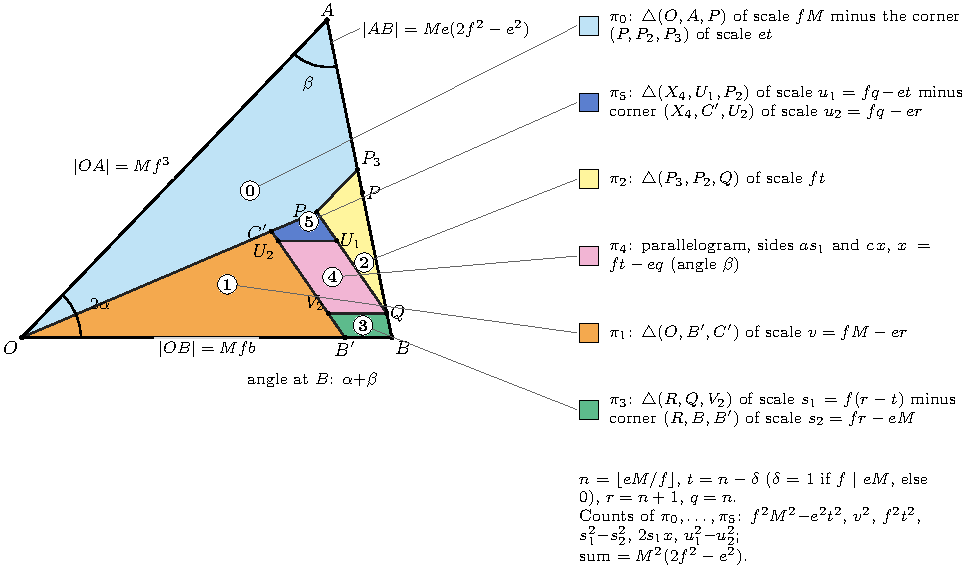
\includegraphics[width=\linewidth]{figures/fig_thmW_schematic_v3.pdf}
\caption{The layout at a glance, with the scales written in the parameters ($n=\lfloor eM/f\rfloor$, $t=n-\delta$, $r=n+1$, $q=n$; $\delta=1$ if $f\mid eM$ and $0$ otherwise). Pieces $0,3,5$ are a triangle minus a corner triangle, piece $4$ is a parallelogram, pieces $1,2$ are triangles (of scales $v$ and $ft$). $O,A,B$ are the vertices of $W_M$; $P$ on $AB$ with $OP=OB$. Drawn with the proportions of $W_3(2,5)$; for the numbers see Example~\ref{ex:414}. The point $R$ (on the line $AB$ beyond $B$) lies outside the drawing.}\label{fig:schematic}
\end{figure}
\emph{What is proved where.}
\begin{center}\small
\begin{tabular}{@{}p{6.1cm}p{6.4cm}@{}}
\toprule
claim & source\\
\midrule
$W_M(e,f)$ is tiled (Thm~\ref{thm:W}) & Lean \lean{thmW} (\texttt{WTilable}) and the hand proof of Section~\ref{sec:proof}\\
$M^2(2f^2-e^2)$, $M^2(3f^2-e^2)$ are tile counts & Lean \lean{thmW}\\
$T_M(e,f)$ is tiled & the glue (I5): Lean, earlier release\\
Sharpness for $e<f/2$ & ``if'': this paper; ``only if'': imported (I1)\\
The layout works iff $M\ge M^*$ (for $M<M^*$) & exhaustive check, $f\le60$ (\CE{}); not proved\\
Explicit tilings ($414$, $656,\dots$) & exact checker (\CE{}), not Lean\\
$26\,138$ new tile counts & computer count (\CE{}); each value is an instance of Theorem~\ref{thm:W}\\
$W_2(5,8)$ & restricted exact search (\CE{}); not formal; no tiling found\\
\bottomrule
\end{tabular}
\end{center}

\subsection{Labels, credit, reading}
Every statement carries a label: \PL{} a theorem of the accompanying Lean~4 library, checked by the kernel with the standard axioms only (\texttt{propext}, \texttt{Classical.choice}, \texttt{Quot.sound}), no \texttt{sorry}; the Lean statement has been compared with the written one \emph{inside this project only}, a reading by an outside person has not been made; \PH{} a written proof, audited inside the project (its polynomial identities are in addition expanded by computer algebra, Appendix~\ref{app:cross}); \CE{} an exact finite computation (for an explicit tiling: exact coordinates and an independent exact checker); \CJ{} unproved.

\emph{Credit and AI.} Credits are in Section~\ref{sec:credit}; the work was done with the help of an AI system (disclosed there).

\emph{Reading.} Ten minutes: this introduction, the symbol table (Table~\ref{tab:notation}; ``Paper~W'' in it means this paper), Figures~\ref{fig:targets} and~\ref{fig:schematic}, and Example~\ref{ex:414}. An hour: Sections~\ref{sec:setting}--\ref{sec:layout}. To check the proof: Section~\ref{sec:proof} and Appendix~\ref{app:cross}; Table~\ref{tab:signs} lists every inequality the proof needs.

%=====================================================================
\section{Setting}\label{sec:setting}

\subsection{The tile}\label{sub:tile}
Throughout, $e<f$ are coprime positive integers and
\[
a=ef,\qquad b=f^2-e^2,\qquad c=f^2,\qquad \kappa=b+c=2f^2-e^2,\qquad d=f-e .
\]
The \emph{tile} $\tile(e,f)$ has sides $a,b,c$ (it is a triangle since $a+b-c=e(f-e)>0$); $\alpha,\beta,\gamma$ are its angles opposite $a,b,c$. One checks $c^2=a^2+bc$ and
\[
3\alpha+2\beta=\pi,\qquad \gamma=2\alpha+\beta,\qquad \cos\alpha=\frac{\kappa}{2c}.
\]
Small examples: $(e,f)=(1,2)$ gives the tile $(2,3,4)$; $(2,3)$ gives $(6,5,9)$; $(2,5)$ gives $(10,21,25)$; $(3,5)$ gives $(15,16,25)$.
\begin{figure}[ht]
\centering
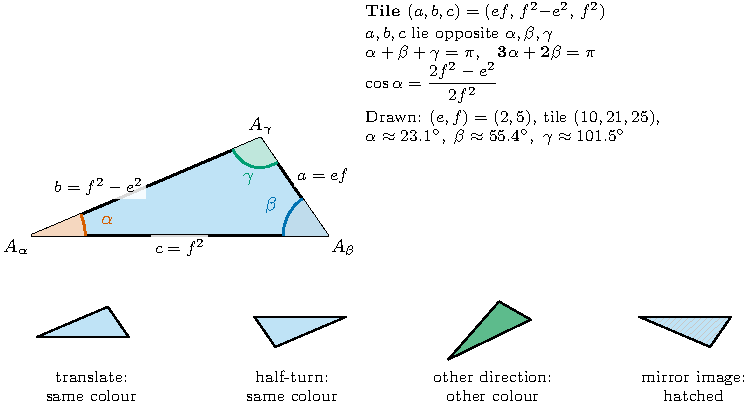
\includegraphics[width=0.8\linewidth]{figures/fig_tile.pdf}
\caption{The tile $\tile(e,f)$ for $(e,f)=(2,5)$, the triangle $(10,21,25)$: sides $a=ef$, $b=f^2-e^2$, $c=f^2$ and angles $\alpha,\beta,\gamma=2\alpha+\beta$ opposite them. The relation $3\alpha+2\beta=\pi$ is what lets the angles of the tile add up to the angles of the targets. In all tiling figures, tiles of the same orientation (up to a half-turn) share a colour and mirror images are hatched.}\label{fig:tile}
\end{figure}

\begin{table}[ht]
\caption{Symbols. This table is shared word for word with the companion paper \cite{Companion}.}\label{tab:notation}
% notation_table.tex -- the ONE notation table shared by Paper W and the companion (version 3.0).  Edit here only.
% [W] = Paper W (Tilings of W_M and T_M below the threshold scale); [C] = the companion paper.
\begin{center}\small
\begin{tabular}{@{}p{2.6cm}p{9.9cm}@{}}
\toprule
symbol & meaning ([W] = Paper W; [C] = the companion paper)\\
\midrule
\multicolumn{2}{@{}l}{\emph{used in both papers}}\\
$e<f$ & coprime positive integers defining the tile; $d=f-e$\\
$a,b,c,\kappa$ & $a=ef$, $b=f^2-e^2$, $c=f^2$, $\kappa=b+c=2f^2-e^2$: the sides of the tile $\tile(e,f)$ and the sum $b+c$\\
$\alpha,\beta,\gamma$ & angles of the tile opposite $a,b,c$; $3\alpha+2\beta=\pi$, $\gamma=2\alpha+\beta$\\
scale $s$ & a triangle with sides $sa,sb,sc$ has \emph{scale} $s$ and is tiled by $s^2$ tiles (ladder subdivision, [W])\\
$W_M$, $T_M$ & the two targets of [W]; $M$ is the \emph{scale} of the target; $W_M$ is tiled by $M^2(2f^2-e^2)$ tiles, $T_M$ by $M^2(3f^2-e^2)$\\
$M^*(e,f)$ & threshold scale $\max(\lceil f/e\rceil,\lceil f/(f-e)\rceil+1)$ of Theorem~W; (H1), (H2) are $Me\ge f$ and $(M-1)(f-e)\ge f$, together equivalent to $M\ge M^*(e,f)$\\
\midrule
\multicolumn{2}{@{}l}{\emph{used in [W] only}}\\
$n,\rho,\delta$ & $n=\lfloor eM/f\rfloor$, $\rho=eM-fn$, $\delta=1$ if $\rho=0$ and $0$ otherwise\\
$t,r,q$ & the three free integers of the six-piece layout; canonical choice $t=n-\delta$, $r=n+1$, $q=n$\\
$\pi_0,\dots,\pi_5$ & the six pieces of the layout; $O,A,B,P,Q,R,\dots$ its points\\
\midrule
\multicolumn{2}{@{}l}{\emph{used in [C] only}}\\
$B_g$ & the isosceles target with base angles $\alpha$; $g$ is its scale; $b\kappa g^2$ tiles\\
row $(e,f)$ & the tile $\tile(e,f)$; $G(e,f)$ is the set of scales $g$ for which $B_g(e,f)$ is tiled\\
$F_0,\dots,F_8$ & the families of Conjecture~C\\
\bottomrule
\end{tabular}
\end{center}

\end{table}

\subsection{The targets}\label{sub:targets}
For an integer $M\ge1$ the two targets of this paper are the triangles
\begin{center}\small
\begin{tabular}{@{}llp{5.4cm}l@{}}
\toprule
target & sides & angles & tiles by area\\
\midrule
$W_M(e,f)$ & $Mfb,\ Me\kappa,\ Mf^3$ & $2\alpha$ (opposite $Me\kappa$), $\beta$ (opposite $Mfb$), $\alpha{+}\beta$ (opposite $Mf^3$) & $M^2(2f^2-e^2)$\\
$T_M(e,f)$ & $Mf^3,\ Mf^3,\ Me(3f^2-e^2)$ & isosceles; apex $3\alpha$, base angles $\beta$ & $M^2(3f^2-e^2)$\\
\bottomrule
\end{tabular}
\end{center}
(Both numbers are the area of the target divided by the area of the tile, so any tiling of the target has exactly that many tiles.) $T_M$ is obtained from $W_M$ by gluing one copy of the tile at scale $Mf$ (sides $Mef^2,\ Mfb,\ Mf^3$) on the side $Mfb$ of $W_M$ (Section~\ref{sub:T}), which is how the $T$ half of Theorem~W is obtained. Both are drawn in Figure~\ref{fig:targets}.
\begin{figure}[ht]
\centering
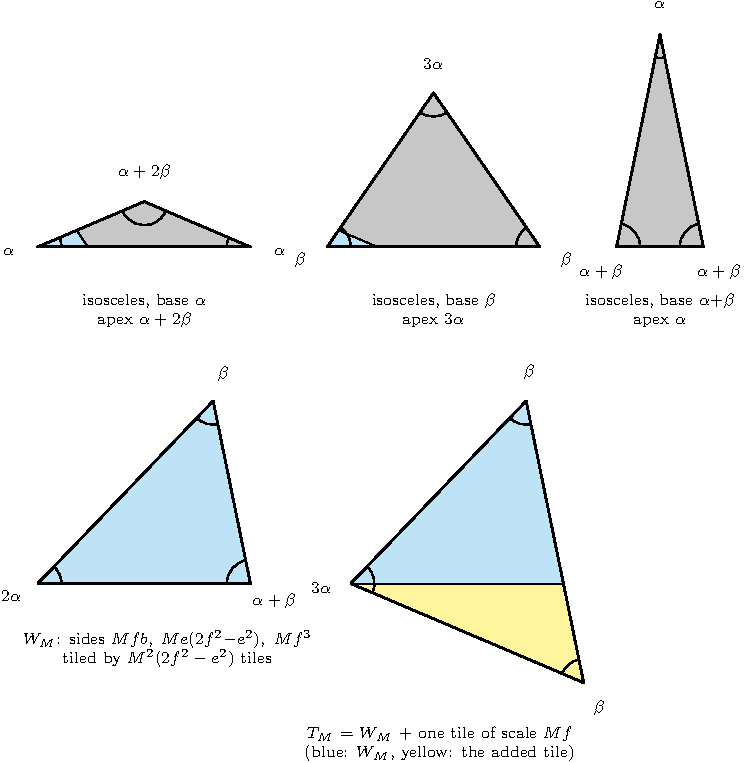
\includegraphics[trim=0 0 0 172bp,clip,width=0.62\linewidth]{figures/fig_targets.pdf}
\caption{The two targets, with the proportions of $(e,f)=(2,5)$, $M=1$. Left: $W_M$ with angles $2\alpha$ (at $O$), $\beta$ (at $A$), $\alpha{+}\beta$ (at $B$), tiled by $M^2(2f^2-e^2)$ tiles. Right: $T_M$, obtained from $W_M$ by adding one tile of scale $Mf$ (yellow) along the side $Mfb$; it is isosceles with apex $3\alpha$ and base angles $\beta$, tiled by $M^2(3f^2-e^2)$ tiles.}\label{fig:targets}
\end{figure}

\subsection{Scale and the ladder}\label{sub:tools}
A triangle with sides $sa,sb,sc$ (similar to the tile) has \emph{scale} $s$.
\begin{proposition}[Ladder subdivision; \PL{}]\label{prop:ladder}
Let $s,u\ge1$ be integers. A triangle of scale $s$ is tiled by $s^2$ copies of $\tile$. A parallelogram with sides $sa$ and $uc$ enclosing the angle $\beta$ is tiled by $2su$ copies of $\tile$.
\end{proposition}
\noindent\emph{Lean:} \lean{Subdivision.ladderDissection}, \lean{Ladder.ladder} (earlier release, \texttt{thm:ladder}). \emph{Why:} a triangle of scale $s$ is cut by the lines parallel to its sides at integer steps into $s^2$ small triangles of scale one, all congruent to the tile (half of them rotated by $\pi$); a parallelogram with sides $a,c$ and angle $\beta$ is two tiles, because its diagonal joining the far ends of the two sides has length $b$.
A \emph{trapezoid} below means a triangle of scale $s_1$ minus a corner triangle of scale $s_2<s_1$ cut off by a line parallel to the opposite side; it is tiled by $s_1^2-s_2^2$ copies (take the tiling of the large triangle by the ladder and remove the $s_2^2$ small triangles of the corner).

\subsection{Coordinates, the sine table, and the points of the layout}\label{sub:pts}
Put $w=\sqrt{4f^2-e^2}$ and write the complex number $\xi+iw\zeta$ ($\xi,\zeta$ rational functions of $e,f$) as $[\xi,\zeta]$. (So $B=fbM$ is the real number $[fbM,0]$.) Then
\[
\varepsilon=e^{i\alpha}=\Bigl[\tfrac{\kappa}{2f^2},\tfrac{e}{2f^2}\Bigr],\qquad
\eta=e^{i\beta}=\Bigl[\tfrac{e(3f^2-e^2)}{2f^3},\tfrac{b}{2f^3}\Bigr],\qquad \omega=\overline{\varepsilon\eta}=e^{-i(\alpha+\beta)} .
\]
Three identities, each checked by clearing denominators and expanding (the first is $3\alpha+2\beta=\pi$):
\[
\varepsilon^3\eta^2=-1\ (\text{this is }3\alpha+2\beta=\pi),\qquad a+b\,\omega=c\,\bar\eta\ (\text{the tile closes up}),\qquad f\omega+e\varepsilon=f\bar\eta .
\]

\emph{Sine table.} For $u,v\in\mathbb C$ put $\langle u,v\rangle=\frac1w\mathrm{Im}(\bar uv)$; it is bilinear over $\mathbb R$, equals $\xi_u\zeta_v-\zeta_u\xi_v$ for $u=[\xi_u,\zeta_u]$, $v=[\xi_v,\zeta_v]$, and is $1/w$ times the usual cross product, hence has the same sign. Every point below is a real combination of the four unit directions $1,\varepsilon,\omega,\bar\eta$, so every cross product in Section~\ref{sec:proof} is obtained by bilinearity from the six numbers
\begin{center}\small
\begin{tabular}{@{}cccccc@{}}
$\langle1,\varepsilon\rangle$ & $\langle1,\omega\rangle$ & $\langle1,\bar\eta\rangle$ & $\langle\varepsilon,\omega\rangle$ & $\langle\varepsilon,\bar\eta\rangle$ & $\langle\omega,\bar\eta\rangle$\\[2pt]
$\dfrac{e}{2f^2}$ & $-\dfrac1{2f}$ & $-\dfrac{b}{2f^3}$ & $-\dfrac1{2f}$ & $-\dfrac1{2f}$ & $\dfrac{e}{2f^2}$
\end{tabular}
\end{center}
(each is read off from the displayed $\varepsilon,\eta,\omega$; for instance $\langle1,\omega\rangle=-\frac1w\mathrm{Im}(\varepsilon\eta)=-\frac{\kappa b+e^2(3f^2-e^2)}{4f^5}=-\frac{2f^4}{4f^5}$). A reader can verify any row of the tables of Appendix~\ref{app:cross} with this table.

Take $O=0$ and the points (vector sums in $\mathbb C$; $M,t,r,q$ the parameters):
\begin{align*}
B&=fbM, & A&=f^3M\varepsilon^2, & P&=fbM\varepsilon,\\
P_2&=b(fM-et)\varepsilon, & P_3&=P-eat\,\omega, & Q&=P+fbt\,\omega, & R&=P+fbr\,\omega,\\
C'&=bv\,\varepsilon, & B'&=cv, & V_2&=P+f^3t\,\bar\eta-ef^2r, & X_4&=P-fbq\,\varepsilon,\\
U_1&=P-ef^2t+ef^2q\,\bar\eta, & U_2&=P-ef^2r+ef^2q\,\bar\eta .
\end{align*}
The triangle $OAB$ has $|OB|=Mfb$, $|OA|=Mf^3$, $|AB|=Me\kappa$ and angles $2\alpha,\beta,\alpha+\beta$ at $O,A,B$: it is $W_M(e,f)$. The point $P$ lies on $AB$ ($A-P=-afM\omega$, $B-P=ebM\omega$) and $|OP|=|OB|$.
The pieces, as ordered vertex lists (counter-clockwise):
\begin{gather*}
\pi_0=(A,O,P_2,P_3),\quad \pi_1=(O,B',C'),\quad \pi_2=(P_3,P_2,Q),\\
\pi_3=(B,Q,V_2,B'),\quad \pi_4=(Q,U_1,U_2,V_2),\quad \pi_5=(U_1,P_2,C',U_2).
\end{gather*}


\subsection{Five facts imported from the earlier release}\label{sub:import}
Five facts about the tile $\tile(e,f)$ and the targets of Section~\ref{sub:targets} are Lean theorems of the earlier release \cite{ReleasePaper,Release22} and are used here as stated, not reproved. \emph{Tiled} always means tiled by copies of $\tile(e,f)$ with the same $(e,f)$.
\begin{enumerate}
\item[(I1)] (\texttt{cor:ebelow}(a), (b), and the case $e=1$) If $Me<f$ then $W_M(e,f)$ is not tiled; if $2Me<f$ then $T_M(e,f)$ is not tiled; for $e=1$, $T_M(1,f)$ is not tiled if $2M\le f$. [All coprime $1\le e<f$.]
\item[(I2)] (\texttt{cor:thickw}(a)) If $M(f-e)\le e$ then $W_M(e,f)$ is not tiled.
\item[(I3)] (\texttt{cor:below}, \texttt{cor:thickw}(b)) For $e=1$ and for $e=f-1$: $W_M(e,f)$ is tiled if and only if $M\ge f$.
\item[(I4)] (Paliy; formalised there) For every $M\ge f$, $W_M(e,f)$ and $T_M(e,f)$ are tiled.
\item[(I5)] (the glue; Lean \lean{CollarG.betaTilable_of_wTilable} and \lean{DebtB.counts_of_wTilable}) If $W_M(e,f)$ is tiled then $T_M(e,f)$ is tiled; and if $W_{M_0}(e,f)$ is tiled and $M_0(f-e)\ge f$, then for every $M\ge M_0$ both $W_M$ and $T_M$ are tiled and $M^2(2f^2-e^2)$, $M^2(3f^2-e^2)$ are tile counts.
\end{enumerate}
The facts are used only outside the proof of the $W$ half: (I1) for the sharpness statement (Corollary~\ref{cor:sharp}) and to say what is open (Section~\ref{sec:open}); (I2), (I3) to say what is open and in Remark~\ref{rem:refute}; (I4) to place the theorem against what was known; (I5) for the $T$ half. The proof of the $W$ half (Sections~\ref{sec:layout}--\ref{sec:proof}) uses none of them.


%=====================================================================
\section{Theorem W and its consequences}\label{sec:thmW}

\subsection{Statement}
\begin{theorem}[Theorem W; $W$ half \PL{} and \PH{}; count of $T_M$ \PL{}; tiling of $T_M$ via the imported glue]\label{thm:W}
Let $e,f$ be coprime integers with $2\le e\le f-2$ and let $M\ge1$ be an integer with
\[
\text{(H1)}\quad Me\ge f,\qquad\qquad \text{(H2)}\quad (M-1)(f-e)\ge f .
\]
Then $W_M(e,f)$ is tiled by $M^2(2f^2-e^2)$ copies of $\tile(e,f)$, and $T_M(e,f)$ is tiled by $M^2(3f^2-e^2)$ copies.
\end{theorem}
Put $M^*(e,f)=\max\bigl(\lceil f/e\rceil,\ \lceil f/(f-e)\rceil+1\bigr)$; then (H1) and (H2) together say $M\ge M^*(e,f)$.
\smallskip

\emph{Exactly what is Lean.} Lean module \texttt{Draft/ThmW.lean} (with 19 helper modules, aggregate \lean{Erdos634.AllThmW}), theorem \lean{Draft.ThmW.thmW}: for natural numbers $e,f,M$ with \texttt{Nat.Coprime e f}, $2\le e$, $e+2\le f$, $f\le M\cdot e$ and $f\le (M-1)\cdot(f-e)$, the conclusion is
\[\texttt{WTilable e f M} \ \wedge\ \texttt{TileCount ((2*f\^{}2-e\^{}2)*M\^{}2)}\ \wedge\ \texttt{TileCount (M\^{}2*(3*f\^{}2-e\^{}2))}.\]
\texttt{WTilable e f M} says: there is a dissection into congruent triangles, each congruent to the triangle with sides $ef,\ f^2-e^2,\ f^2$, of a triangle with sides $Mf(f^2-e^2)$, $Me(2f^2-e^2)$, $Mf^3$. So Lean states the \emph{tiling} for $W_M$; for $T_M$ it states only that the number is a tile count, and the tiling of $T_M$ itself is the glue (I5), a Lean theorem of the earlier release (Section~\ref{sub:T}). Axioms: \texttt{propext}, \texttt{Classical.choice}, \texttt{Quot.sound}. The Lean statement was compared with the one above inside the project (verdict: match; a note on credits in nine module headers). Hypotheses are witnessed by instances \lean{inst_414}, \lean{inst_656}, \lean{inst_801} (and others), so the Lean theorem is not vacuous.
The hand proof is Sections~\ref{sec:layout}--\ref{sec:proof} with Appendix~\ref{app:cross}; Section~\ref{sub:checked} lists what is checked how.


First instances, by $e,f$ (the last column is the smallest scale for which a tiling was known before this paper, namely $f$; the scale of the newly tiled target is in column 3):
\begin{center}\small
\begin{tabular}{@{}lllll@{}}
\toprule
$(e,f)$ & $M^*$ & first tiled $W_{M^*}$ & number of tiles & smallest $M$ known before\\
\midrule
$(2,5)$ & $3$ & $W_3(2,5)$ & $414$ & $5$\\
$(3,5)$ & $4$ & $W_4(3,5)$ & $656$ & $5$\\
$(3,7)$ & $3$ & $W_3(3,7)$ & $801$ & $7$\\
$(2,11)$ & $6$ & $W_6(2,11)$ & $8568$ & $11$\\
$(9,11)$ & $7$ & $W_7(9,11)$ & $7889$ & $11$\\
\bottomrule
\end{tabular}
\end{center}
Thirteen targets with $M<f$ were found by a bounded computer search before the proof was known (Appendix~\ref{app:data}); they are only the output of that one search, not a list of all instances. The theorem has many more instances with $M<f$, for example $(e,f,M)=(4,9,3)$ and $(3,8,3)$.

\subsection{Consequences}
\begin{corollary}[Sharpness for $e<f/2$; ``if'': Theorem~\ref{thm:W} \PL{} plus the arithmetic below; ``only if'': the imported (I1)]\label{cor:sharp}
Let $\gcd(e,f)=1$ and $2\le e<f/2$. Then $W_M(e,f)$ is tiled if and only if $Me\ge f$.
\end{corollary}
\begin{proof}
``Only if'' is (I1). ``If'': $e<f/2$ gives $f-e>f/2$, so $f/(f-e)<2$ and $\lceil f/(f-e)\rceil+1=3$, while $f/e>2$ gives $\lceil f/e\rceil\ge3$; so $M^*=\lceil f/e\rceil$. Moreover (H1) implies (H2): (H1) gives $M\ge3$, so $(M-1)(f-e)\ge2(f-e)>f$. Apply Theorem~\ref{thm:W}.
\end{proof}
For $e<f/2$ the threshold is therefore \emph{exactly} $\lceil f/e\rceil$, which is smaller than $f$ as soon as $e\ge2$. (For $e=1$ it is $f$, by (I3).) The ``only if'' half is not proved in this paper; it is only as strong as the import (I1).
\begin{corollary}[An open case; \PL{} for the tiling, \CE{} for the data]\label{cor:W435}
$W_4(3,5)$, a triangle with sides $320,\,492,\,500$, is tiled by $656$ copies of $(15,16,25)$.
\end{corollary}
\noindent This is Theorem~\ref{thm:W} for $(e,f,M)=(3,5,4)$ ($M^*(3,5)=\max(2,4)=4$). A list of the $656$ tiles in exact coordinates is shipped (Appendix~\ref{app:data}) and verified by an exact checker.

\begin{remark}[Two earlier expectations that are false]\label{rem:refute}
(a) \emph{The threshold conjecture ``B1''.} Our earlier notes expected that, for $e\ge2$, neither $W_M$ nor $T_M$ is tiled for $M<f$; the earlier paper \cite{ReleasePaper} recorded as an observation that every case decided so far has threshold $f$, and listed $W_4(3,5)$ among the open cases. Corollary~\ref{cor:W435} is a counterexample ($4<5$), and Theorem~\ref{thm:W} gives infinitely many.
(b) \emph{The size conjecture.} The notes also stated that a target not similar to the tile has longest side at least $c^2=f^4$. For $W_4(3,5)$ the longest side is $500<625=c^2$.
Neither statement was published as a theorem or is part of any Lean statement; they were expectations of our working notes (the first also appears as an observation and an open case in \cite{ReleasePaper}), and no earlier theorem is affected.
\end{remark}

\subsection{The $T$ half}\label{sub:T}
Glue to the side $Mfb$ of $W_M$ (the side from $O$ to $B$ in Section~\ref{sec:layout}) one copy of the tile at scale $Mf$, with its side $Mfb$ on that side and its third vertex $Z$ on the line $AB$ beyond $B$, so that $BZ=Mef^2$. The result is the isosceles triangle with legs $Mf^3$ and base $Me(3f^2-e^2)$, that is $T_M$, and its tile count is $M^2(2f^2-e^2)+(Mf)^2=M^2(3f^2-e^2)$.
This is (I5). The Lean theorem \lean{Draft.ThmW.thmW} contains the \emph{count} for $T_M$, obtained from the tiling of $W_M$ by \lean{DebtB.counts_of_wTilable}, which needs besides the tiling only $M(f-e)\ge f$; (H2) implies it.
The converse (a tiling of $T_M$ gives one of $W_M$) is not known, and the proved exclusions for $T_M$ are weaker ((I1): only $2Me<f$). Hence the label of the $T$ half is: tiling of $W_M$ \PL{}\,\PH{}; tile count of $T_M$ \PL{}; tiling of $T_M$ by the imported glue \PL{} in the earlier release.

%=====================================================================
\section{The six-piece layout}\label{sec:layout}

\subsection{The idea, then the table}\label{sub:idea}
The target $W_M(e,f)$ has a vertex $O$ with angle $2\alpha$ and two other vertices $A$ (angle $\beta$) and $B$ (angle $\alpha+\beta$); the sides are $|OB|=Mfb$, $|OA|=Mf^3$, $|AB|=Me\kappa$.
Let $P$ be the point of $AB$ with $OP=OB$. The triangle $OBP$ is isosceles with base angles $\alpha+\beta$ (at $B$ and $P$), so its angle at $O$ is $\pi-2(\alpha+\beta)=\alpha$ (because $3\alpha+2\beta=\pi$); hence $\angle AOP=2\alpha-\alpha=\alpha$ and $OP$ bisects the angle at $O$. The triangle $OAP$ has sides $OP=fb\,M$ and $OA=cf\,M$ enclosing the angle $\alpha$, the two sides of a tile (sides $b$ and $c$ enclose $\alpha$): \emph{$OAP$ has scale $fM$}, an integer.
This is the whole idea: the big triangle $OAP$ is cut off first, and what remains is the thin quadrilateral-like region along $AB$ and $OB$ near $B$, which is filled by five further pieces of integer scale.
Figure~\ref{fig:schematic} (in the introduction) shows the layout with its parameters in symbols, Table~\ref{tab:pieces} gives the pieces, and Example~\ref{ex:414} the numbers for $W_3(2,5)$.

\emph{Points} (coordinates in Section~\ref{sub:pts}). All points lie in the plane of $OAB$; $a,b,c$ are the tile sides; $OB$ is taken as the positive real axis, $\varepsilon$ is the unit vector along $OP$ (angle $\alpha$ from $OB$), $\omega$ the unit vector along $AB$ from $A$ to $B$, and $\bar\eta$ the unit vector at angle $-\beta$ (all made precise in Section~\ref{sub:pts}). The points of Table~\ref{tab:pieces} are:
\begin{center}\small
\begin{tabular}{@{}lp{10.6cm}@{}}
\toprule
point & description\\
\midrule
$P$ & on $AB$ with $OP=OB$ (so $OP$ bisects $\angle O$)\\
$P_2$ & on $OP$ at distance $b\,et$ from $P$; $\quad P_3$ on $PA$ at distance $a\,et$ from $P$\\
$Q,\ R$ & on line $AB$ beyond $P$ towards $B$, at distances $fb\,t$ and $fb\,r$ from $P$ ($R$ lies beyond $B$)\\
$B'$ & on $OB$ with $OB'=c\,v$; $\quad C'$ on $OP$ with $OC'=b\,v$\\
$V_2$ & $Q$ moved by $a\,s_1$ in the direction of $OB$ reversed (so $QV_2\parallel OB$)\\
$U_1,\ U_2$ & $U_1=Q+c\,x\,\mathbf u$, $U_2=V_2+c\,x\,\mathbf u$, where $\mathbf u$ is the unit vector of the side $c$ of the tile at the angle $\beta$ ($\mathbf u=-\bar\eta$)\\
$X_4$ & on $OP$ at distance $fb\,q$ from $P$ towards $O$ (the corner of the triangle of $\pi_5$)\\
\bottomrule
\end{tabular}
\end{center}
The layout depends on the target scale $M$ and on three further integers $t,r,q\ge1$ (to be chosen); put
\[
v=fM-er,\quad s_1=f(r-t),\quad s_2=fr-eM,\quad x=ft-eq,\quad u_1=fq-et,\quad u_2=fq-er .
\]
\begin{table}[ht]
\caption{The six pieces. Each is tiled by Proposition~\ref{prop:ladder}; the last column is the number of tiles. The points are defined in Section~\ref{sub:pts}.}\label{tab:pieces}
\centering\small
\begin{tabular}{@{}llp{7.3cm}l@{}}
\toprule
piece & kind & description & tiles\\
\midrule
$\pi_0$ & trapezoid & triangle $OAP$ (scale $fM$) minus its corner at $P$ of scale $et$ & $f^2M^2-e^2t^2$\\
$\pi_1$ & triangle & $OB'C'$, scale $v$ & $v^2$\\
$\pi_2$ & triangle & $P_3P_2Q$, scale $ft$ & $f^2t^2$\\
$\pi_3$ & trapezoid & triangle $RQV_2$ (scale $s_1$) minus its corner at $R$ of scale $s_2$ & $s_1^2-s_2^2$\\
$\pi_4$ & parallelogram & sides $a\,s_1$ and $c\,x$, angle $\beta$ & $2s_1x$\\
$\pi_5$ & trapezoid & triangle $X_4U_1P_2$ (scale $u_1$) minus its corner at $X_4$ of scale $u_2$ & $u_1^2-u_2^2$\\
\bottomrule
\end{tabular}
\end{table}
The six counts add up to $M^2(2f^2-e^2)$ \emph{identically} in $e,f,M,t,r,q$ (a polynomial identity, expanded by computer algebra; Section~\ref{sub:checked}), so the area is automatic. What remains is (i) that the scales are positive integers and (ii) that the pieces lie inside $OAB$ and do not overlap: a finite list of inequalities, Table~\ref{tab:signs}.
The proof chooses
\[
n=\Bigl\lfloor \frac{eM}{f}\Bigr\rfloor,\qquad \rho=eM-fn\in[0,f),\qquad \delta=\begin{cases}1&\rho=0\\0&\rho>0\end{cases},\qquad
t=n-\delta,\quad r=n+1,\quad q=n,
\]
and shows that under (H1), (H2) every inequality holds. (H1) enters through $n\ge1$, (H2) through $M-n\ge2$ and $dM\ge f+d$.
\emph{Why these values.} $r=n+1$ is the smallest integer with $fr>eM$ (so that $R$ lies beyond $B$ and $s_2>0$); $t=n-\delta$ is the largest integer with $ft<eM$ (recall $eM=fn+\rho$; so that the corner piece $\pi_2$ is as large as the layout allows, which leaves the three small pieces thin); $q=n$ is a convenient integer in the window $er<fq$, $eq<ft$ that the remaining pieces need (other values may also work; none is needed). The proof does not depend on how the values were found.



\emph{Where the pieces sit.} Walking along $AB$ from $A$: first $\pi_0$ (to $P_3$), then $\pi_2$ ($P_3$ to $Q$, passing $P$), then $\pi_3$ ($Q$ to $B$). Along $OB$ from $B$: $\pi_3$ (to $B'$), then $\pi_1$ (to $O$). Along $OA$: only $\pi_0$. The two big pieces $\pi_0$ and $\pi_1$ meet along the line $OP_2C'$ (the bisector $OP$ shortened); between $\pi_2$ on one side and $\pi_1$, $\pi_0$ on the other lies a strip, filled from the top by $\pi_5$, then $\pi_4$, with $\pi_3$ closing the bottom (Figure~\ref{fig:zoom}). So the layout is: two big pieces, two thin pieces on the sides ($\pi_2,\pi_3$), and a two-piece strip between them.

\subsection{Worked examples}\label{sub:examples}
\begin{example}[$W_3(2,5)$, $414$ tiles]\label{ex:414}
$(e,f,M)=(2,5,3)$: $a=10$, $b=21$, $c=25$, $\kappa=46$; $W_3(2,5)$ has sides $Mfb=315$, $Me\kappa=276$, $Mf^3=375$.
$n=\lfloor 6/5\rfloor=1$, $\rho=1$, $\delta=0$, so $(t,r,q)=(1,2,1)$ and $v=11$, $s_1=5$, $s_2=4$, $x=3$, $u_1=3$, $u_2=1$.
\begin{center}\small
\begin{tabular}{@{}lccc@{\qquad}lccc@{}}
\toprule
 & scales & formula & tiles & & scales & formula & tiles\\
\midrule
$\pi_0$ & $15$ minus $2$ & $225-4$ & $221$ & $\pi_3$ & $5$ minus $4$ & $25-16$ & $9$\\
$\pi_1$ & $11$ & $11^2$ & $121$ & $\pi_4$ & $as_1\times cx$ & $2\cdot5\cdot3$ & $30$\\
$\pi_2$ & $5$ & $5^2$ & $25$ & $\pi_5$ & $3$ minus $1$ & $9-1$ & $8$\\
\bottomrule
\end{tabular}
\end{center}
Total $221+121+25+9+30+8=414=9\cdot46=M^2(2f^2-e^2)$. The tiling is drawn in Figure~\ref{fig:template} (the numbers in the circles are the piece numbers of Table~\ref{tab:pieces}); a list of the $414$ tiles in exact coordinates is shipped and verified by an exact checker.
\end{example}
\begin{figure}[ht]
\centering
\begin{tikzpicture}[x=1bp,y=1bp]
\node[anchor=south west,inner sep=0] (m) at (0,0) {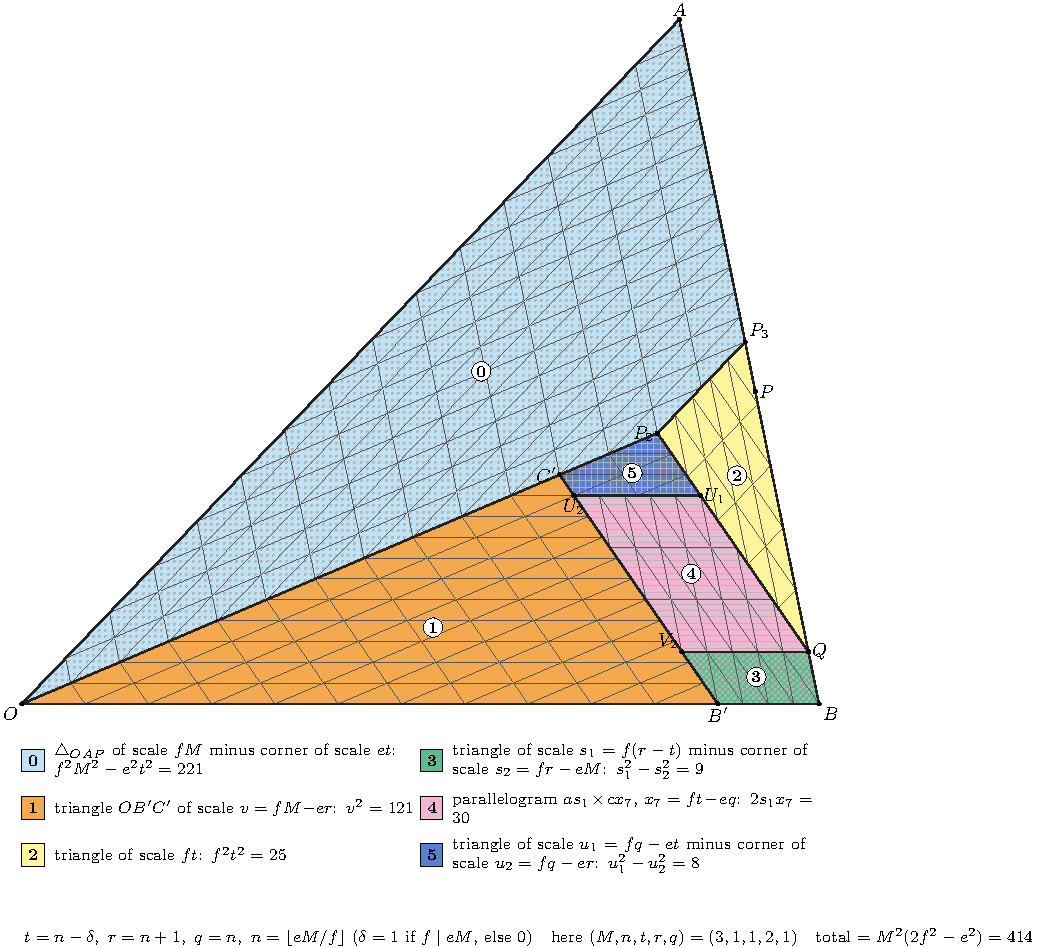
\includegraphics[trim=0 100bp 0 0,clip,width=380bp]{figures/fig_thmW_template.pdf}};
\draw[red!70!black,thick] (0.4698*380,380/500.258*5) rectangle (0.8196*380,380/500.258*207);
\end{tikzpicture}
\caption{The layout for $W_3(2,5)$ (tile $(10,21,25)$, $414$ tiles, $(M,n,t,r,q)=(3,1,1,2,1)$). Colours are pieces, numbered $0$--$5$ as in Table~\ref{tab:pieces} ($0$ light blue, $1$ orange, $2$ yellow, $3$ green, $4$ pink, $5$ dark blue); the thin lines are the $414$ tiles of the exact tiling. The large pieces $\pi_0$ and $\pi_1$ carry $342$ of the $414$ tiles; the four small pieces lie in the red box and are enlarged in Figure~\ref{fig:zoom}.}\label{fig:template}
\end{figure}
\begin{figure}[ht]
\centering
\scalebox{0.72}{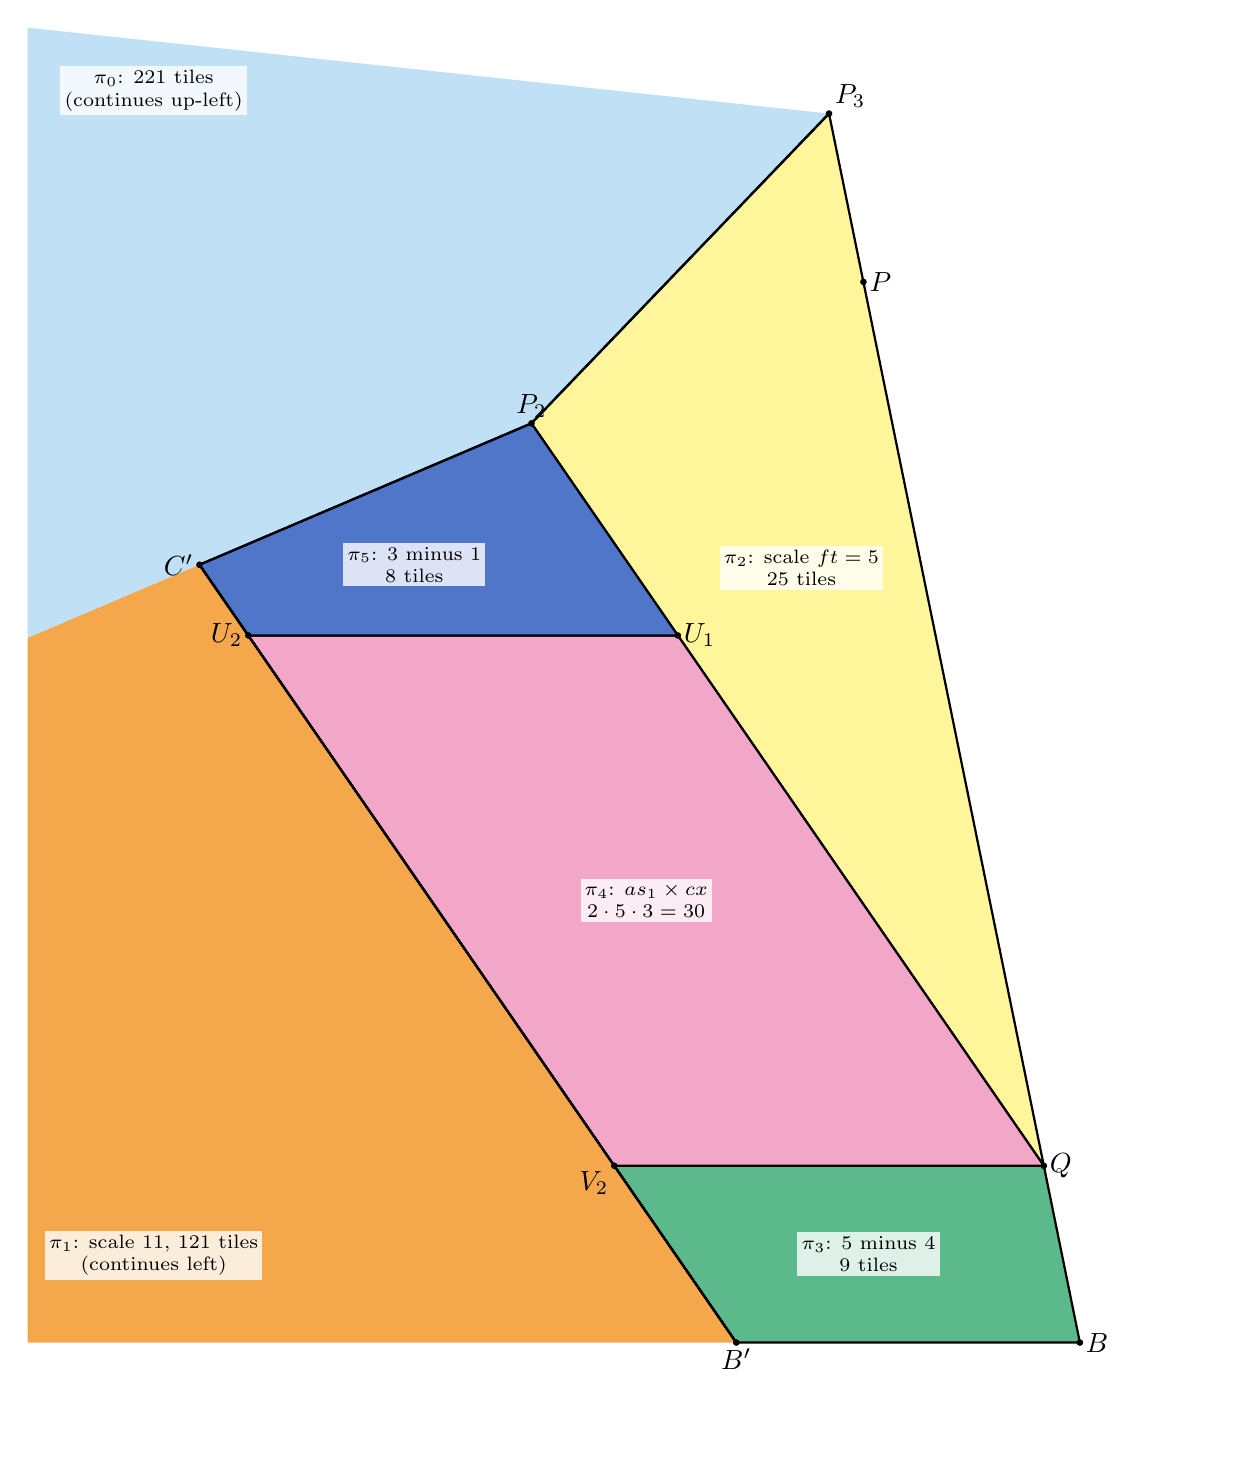
\begin{tikzpicture}[x=1cm,y=1cm,font=\footnotesize]
\definecolor{ef1}{HTML}{F4A74B}\definecolor{ef2}{HTML}{BFE0F5}\definecolor{ef3}{HTML}{5BB98C}\definecolor{ef4}{HTML}{FFF59A}\definecolor{ef5}{HTML}{4F76C9}\definecolor{ef7}{HTML}{F2A7C9}
\begin{scope}\clip (0,0) rectangle (15.000,17.790);
\fill[ef2] (10.177,16.699) -- (6.398,12.765) -- (0,10.039) -- (0,17.790) -- cycle;
\fill[ef1] (8.999,1.091) -- (2.182,10.969) -- (0,10.039) -- (0,1.091) -- cycle;
\fill[ef4,draw=black,line width=0.8pt] (10.177,16.699) -- (6.398,12.765) -- (12.905,3.336) -- cycle;
\fill[ef3,draw=black,line width=0.8pt] (13.363,1.091) -- (12.905,3.336) -- (7.450,3.336) -- (8.999,1.091) -- cycle;
\fill[ef7,draw=black,line width=0.8pt] (12.905,3.336) -- (8.257,10.071) -- (2.802,10.071) -- (7.450,3.336) -- cycle;
\fill[ef5,draw=black,line width=0.8pt] (8.257,10.071) -- (6.398,12.765) -- (2.182,10.969) -- (2.802,10.071) -- cycle;
\draw[line width=0.8pt] (10.177,16.699) -- (6.398,12.765); \draw[line width=0.8pt] (8.999,1.091) -- (2.182,10.969);
\draw[line width=0.8pt] (6.398,12.765) -- (2.182,10.969) -- (8.999,1.091);
\end{scope}
\fill (10.177,16.699) circle (1.2pt); \node[above right,inner sep=2pt] at (10.177,16.699) {\normalsize$P_3$};
\fill (6.398,12.765) circle (1.2pt); \node[above,inner sep=2pt] at (6.398,12.765) {\normalsize$P_2$};
\fill (12.905,3.336) circle (1.2pt); \node[right,inner sep=2pt] at (12.905,3.336) {\normalsize$Q$};
\fill (13.363,1.091) circle (1.2pt); \node[right,inner sep=2pt] at (13.363,1.091) {\normalsize$B$};
\fill (8.999,1.091) circle (1.2pt); \node[below,inner sep=2pt] at (8.999,1.091) {\normalsize$B'$};
\fill (2.182,10.969) circle (1.2pt); \node[left,inner sep=2pt] at (2.182,10.969) {\normalsize$C'$};
\fill (7.450,3.336) circle (1.2pt); \node[below left,inner sep=2pt] at (7.450,3.336) {\normalsize$V_2$};
\fill (8.257,10.071) circle (1.2pt); \node[right,inner sep=2pt] at (8.257,10.071) {\normalsize$U_1$};
\fill (2.802,10.071) circle (1.2pt); \node[left,inner sep=2pt] at (2.802,10.071) {\normalsize$U_2$};
\fill (10.614,14.561) circle (1.2pt); \node[right,inner sep=2pt] at (10.614,14.561) {\normalsize$P$};
\node[align=center,fill=white,fill opacity=0.8,text opacity=1,inner sep=1.5pt,font=\scriptsize] at (9.827,10.933) {$\pi_2$: scale $ft=5$\\$25$ tiles};
\node[align=center,fill=white,fill opacity=0.8,text opacity=1,inner sep=1.5pt,font=\scriptsize] at (10.679,2.214) {$\pi_3$: $5$ minus $4$\\$9$ tiles};
\node[align=center,fill=white,fill opacity=0.8,text opacity=1,inner sep=1.5pt,font=\scriptsize] at (7.854,6.703) {$\pi_4$: $as_1\times cx$\\$2\cdot5\cdot3=30$};
\node[align=center,fill=white,fill opacity=0.8,text opacity=1,inner sep=1.5pt,font=\scriptsize] at (4.910,10.969) {$\pi_5$: $3$ minus $1$\\$8$ tiles};
\node[align=center,fill=white,fill opacity=0.8,text opacity=1,inner sep=1.5pt,font=\scriptsize] at (1.600,16.990) {$\pi_0$: $221$ tiles\\(continues up-left)};
\node[align=center,fill=white,fill opacity=0.8,text opacity=1,inner sep=1.5pt,font=\scriptsize] at (1.600,2.200) {$\pi_1$: scale $11$, $121$ tiles\\(continues left)};
\end{tikzpicture}}
\caption{Enlargement of the red box of Figure~\ref{fig:template} (exact coordinates of $W_3(2,5)$, drawn to scale; the points $R$ and $X_4$ of Section~\ref{sub:pts} lie outside the box): the four small pieces $\pi_2$ (yellow), $\pi_5$ (dark blue), $\pi_4$ (pink), $\pi_3$ (green) and the edges of $\pi_0$ and $\pi_1$ near them, with all the points of Section~\ref{sub:pts} that lie in the box. Each small piece is a triangle, a triangle minus a corner, or a parallelogram of Table~\ref{tab:pieces}; its scale and tile count are written inside ($P$ is the point of $AB$ with $OP=OB$).}\label{fig:zoom}
\end{figure}
\begin{example}[$W_4(3,5)$, $656$ tiles: below the old threshold, $M=4<5=f$]\label{ex:656}
$(e,f,M)=(3,5,4)$: $a=15$, $b=16$, $c=25$, $\kappa=41$; $n=\lfloor12/5\rfloor=2$, $\rho=2$, $\delta=0$, $(t,r,q)=(2,3,2)$; $v=11$, $s_1=5$, $s_2=3$, $x=4$, $u_1=4$, $u_2=1$; counts $364+121+100+16+40+15=656=16\cdot41$. See Figure~\ref{fig:small}.
\end{example}
\begin{figure}[ht]
\centering
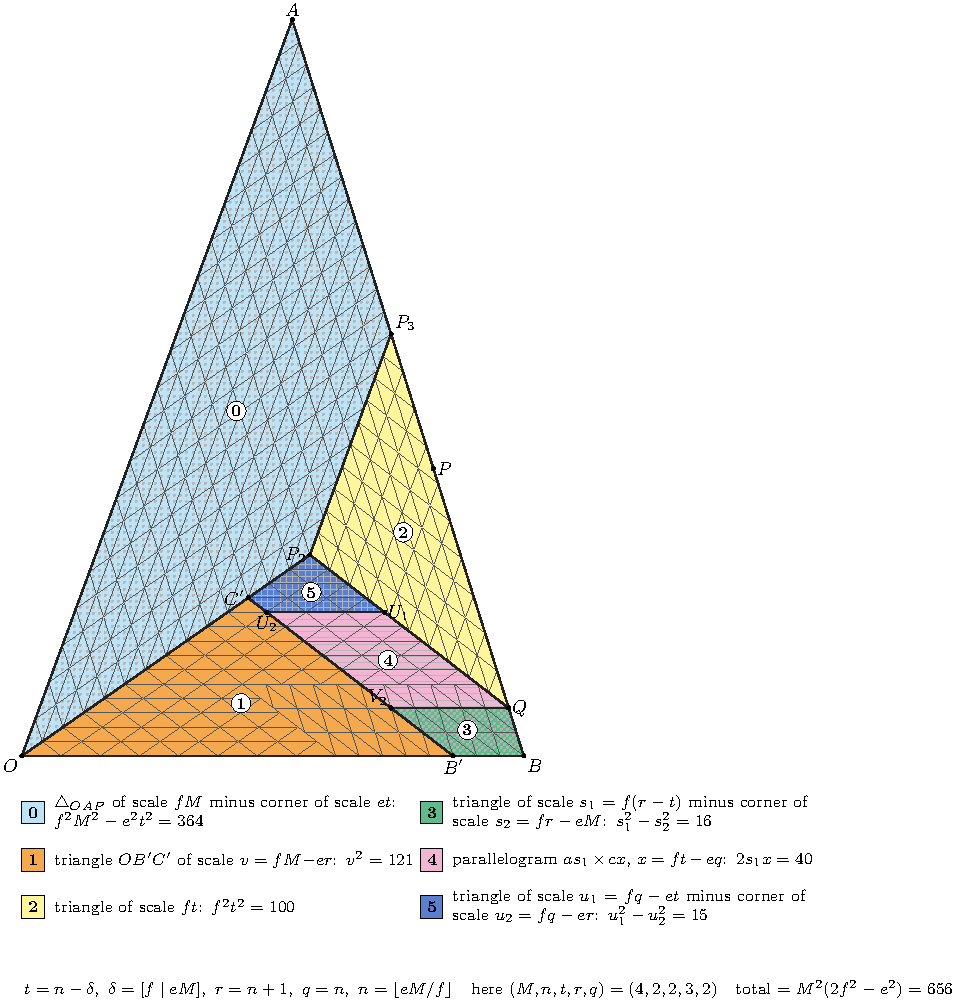
\includegraphics[width=0.85\linewidth]{figures/fig_thmW_small_v3.pdf}
\caption{The same layout for $W_4(3,5)$ ($656$ tiles of $(15,16,25)$, $(M,n,t,r,q)=(4,2,2,3,2)$). Colours and numbers as in Figure~\ref{fig:template}; counts $364+121+100+16+40+15$.}\label{fig:small}
\end{figure}
\begin{example}[the case $\delta=1$: $(e,f,M)=(2,5,5)$, $M=f$]\label{ex:delta}
Here $f\mid eM$: $n=2$, $\rho=0$, $\delta=1$, so $(t,r,q)=(1,3,2)$ and $v=19$, $s_1=10$, $s_2=5$, $x=1$, $u_1=8$, $u_2=4$; counts $621+361+25+75+20+48=1150=25\cdot46$.
\end{example}
\begin{example}[a failing choice: $(e,f,M)=(3,5,3)$]\label{ex:fail}
$M^*(3,5)=4$ and (H2) fails ($2\cdot2=4<5$). The canonical parameters are $(t,r,q)=(1,2,1)$; with them the scale $u_2=fq-er=5-6=-1$ of $\pi_5$ is negative and all other scales are positive. So the layout with the canonical parameters does not exist here; this does not show that $W_3(3,5)$ is untiled (it is an open case, Section~\ref{sec:open}).
\end{example}

%=====================================================================
\section{Proof of Theorem~W}\label{sec:proof}
\emph{Outline.} (1) Write the six pieces with explicit coordinates (Section~\ref{sub:pts}). (2) Show each is a union of tiles when its scales are positive integers (Section~\ref{sub:shapes}). (3) Show that the pieces lie in the target and do not overlap, which reduces to the positivity of the named factors (Section~\ref{sub:placement}); all $15$ pairs of pieces are handled: $\pi_0$ against each of $\pi_1,\dots,\pi_5$ (edges $OP_2$ or $P_2P_3$), $\pi_1$ against $\pi_2,\dots,\pi_5$ (edge $B'C'$), $\pi_2$ against $\pi_3,\pi_4,\pi_5$ (edge $P_2Q$), $\pi_3$ against $\pi_4,\pi_5$ (edge $QV_2$), $\pi_4$ against $\pi_5$ (edge $U_1U_2$). (4) Prove the positivity for the canonical parameters (Section~\ref{sub:params}); this is where (H1), (H2) are used. The area identity then finishes the proof. Steps (1)--(2) and the identities are routine and machine-checked; step (3) reduces to a finite table; step (4) is the real content, and the five conditions marked $\ast$ in Table~\ref{tab:signs} carry the real content (the others follow from (P1)--(P3) or are sums of positive terms).
Standing assumptions: $e,f$ coprime, $2\le e\le f-2$, $d=f-e\ge2$.

\subsection{Step 1: shapes}\label{sub:shapes}
\emph{Claim.} If $s_1>s_2>0$, $u_1>u_2>0$, $v>0$, $ft>0$, $x>0$ and $fM>et$, then each piece is the union of the stated number of tiles.
Each item below is a vector identity in $\mathbb C$, i.e.\ a polynomial identity in $e,f,M,t,r,q$ after clearing denominators.
\begin{itemize}\itemsep1pt
\item $\pi_0$: $OP=bfM\varepsilon$ and $OA=cfM\varepsilon^2$ have lengths $bfM$, $cfM$ and enclose $\alpha$, so $OAP$ has scale $fM$ (SAS). The points $P_2\in OP$, $P_3\in PA$ satisfy $PP_2:PO=PP_3:PA=et:fM$, so $P_2P_3\parallel OA$ and the cut-off corner has scale $et$.
\item $\pi_1$: $OB'=cv$ and $OC'=bv\varepsilon$ enclose $\alpha$: scale $v$.
\item $\pi_2$: $Q-P_3=(ea+fb)t\,\omega=f^3t\,\omega$ has length $c\cdot ft$, and $|P_3P_2|=c\cdot et=a\cdot ft$; the angle at $P_3$ is the angle $\beta$ of the corner triangle $PP_2P_3$ (similar to $OPA$): scale $ft$.
\item $\pi_3$: $Q-V_2=a s_1$ is real (the closing identity times $ft$); $R-Q=bs_1\omega$; the angle at $Q$ between $\omega$ and $-1$ is $\gamma$; so $RQV_2$ has scale $s_1$. $B$ lies on $RQ$ and $B'$ on $RV_2$ with $RB:RQ=RB':RV_2=s_2:s_1$ (the corner at $R$ has scale $s_2$).
\item $\pi_4$: $U_1-Q=-f^2x\,\bar\eta=U_2-V_2$, so $QU_1U_2V_2$ is a parallelogram with sides $as_1$, $cx$ and angle $\beta$.
\item $\pi_5$: $P_2-X_4=bu_1\varepsilon$, $|U_1-X_4|=cu_1$, $|U_1-P_2|=au_1$: scale $u_1$; $C'$ lies on $X_4P_2$ and $U_2$ on $X_4U_1$ with ratio $u_2:u_1$.
\end{itemize}
By Proposition~\ref{prop:ladder} each piece is tiled; counts are those of Table~\ref{tab:pieces}.

\subsection{Step 2: placement reduces to a table of signs}\label{sub:placement}
Recall $\langle u,v\rangle$ from Section~\ref{sub:pts} (a positive multiple of the usual cross product). All six pieces are convex and counter-clockwise: the consecutive cross products of each piece are positive constants times a product of the scales (Appendix~\ref{app:cross}, Table~\ref{tab:conv}), and the doubled signed area of piece $i$ is $\frac{eb}{2}$ times its tile count.
\begin{lemma}[covering]\label{lem:cover}
Let $\Omega$ be a closed convex polygon and $\Pi_1,\dots,\Pi_k\subset\Omega$ closed convex polygons whose areas add up to the area of $\Omega$. If for every pair $i<j$ some edge line of $\Pi_i$ (or of $\Pi_j$) has the other polygon on its closed outer side, then the interiors are pairwise disjoint and $\bigcup\Pi_i=\Omega$.
\end{lemma}
\emph{Proof.} A line with $\Pi_i$ on one closed side and $\Pi_j$ on the other closed side separates the interiors, so they are disjoint; hence the union has area $\sum\mathrm{area}(\Pi_i)=\mathrm{area}(\Omega)$. The union is closed and contained in $\Omega$; if it missed a point of $\Omega$, it would miss a relatively open subset of $\Omega$, which has positive area. So the union is $\Omega$. $\square$\\
Hence a piece lies in the triangle $OAB$ iff its vertices do, i.e.\ iff $\langle B-O,Z-O\rangle$, $\langle A-B,Z-B\rangle$, $\langle O-A,Z-A\rangle\ge0$ for every vertex $Z$ (the three sides of $OAB$).
Two pieces have disjoint interiors if some edge line of one has the other piece on its closed outer side. The edges used are
\[
\begin{array}{ll}
\pi_0|\pi_1: OP_2,&\quad \pi_0|\pi_2: P_2P_3,\qquad \pi_0|\{\pi_3,\pi_4,\pi_5\}: OP_2,\\
\pi_1|\ast: B'C',&\quad \pi_2|\ast: P_2Q,\qquad \pi_3|\{\pi_4,\pi_5\}: QV_2,\qquad \pi_4|\pi_5: U_1U_2 .
\end{array}
\]
\emph{Named factors} (the vertex $C'$ and the factors $C_3',C_6'$ are unrelated; primes mark a second factor of the same family).  Write $C_2=r-t$, $C_3=eM-ft$, $C_3'=fM-et$, $C_4=fr-eM$, $C_5=fM-er$, $C_6=fq-er$, $C_6'=fq-et$, $C_7=ft-eq$, $C_8=f^2t-e^2r$, $C_9=fr-eq$, $C_{10}=M-q$; $E_1=bM+eft$, $E_2=eMf+bt$, $E_3=br+e^2t$; and $L_A=bfM-e\kappa t+f^3q$, $L_B=bfM-e\kappa r+f^3q$, $L_C=efbM-e^2\kappa r+f^4t$ (Table~\ref{tab:signs}). The scales are $v=C_5$, $s_1=fC_2$, $s_2=C_4$, $s_1-s_2=C_3$, $x=C_7$, $u_1=C_6'$, $u_2=C_6$, $u_1-u_2=eC_2$. The conditions with real content are $C_6,C_7,C_8,L_B,L_C$ (marked $\ast$ in Table~\ref{tab:signs}); the others follow directly from (P1)--(P3) or are sums of positive terms.
\emph{Fact} (bilinear expansion with the sine table, done by computer algebra in Appendix~\ref{app:cross}; each row can be redone by hand). Each of these cross products, for each vertex of the other piece, and each containment cross product, is equal to a positive rational constant times a product of the \emph{named factors} of Table~\ref{tab:signs} (the Tables of Appendix~\ref{app:cross} show every factorisation). So the whole placement question is: \emph{are the named factors positive?}
\emph{One row by hand.} Separation $\pi_0|\pi_1$ at the vertex $B'$: the edge vector is $u=P_2-O=b(fM-et)\varepsilon$ and $B'-O=cv=f^2v$ is real, so $\langle u,B'-O\rangle=\frac1w\mathrm{Im}(\bar u\,f^2v)=-b(fM-et)f^2v\cdot\frac{e}{2f^2}=-\tfrac{eb}{2}(fM-et)\,v$ (using $\frac1w\mathrm{Im}\,\varepsilon=\frac{e}{2f^2}$); its negative is $\frac12\,e\,b\,C_3'\,C_5$, the first row of Table~\ref{tab:sep}. 
\emph{A containment row by hand.} Vertex $Q$ against the side $OB$: with $\frac1w\mathrm{Im}\,\omega=-\frac1{2f}$ (because $\frac1w\mathrm{Im}(\varepsilon\eta)=\frac{\kappa b+e^2(3f^2-e^2)}{4f^5}=\frac{2f^4}{4f^5}=\frac1{2f}$) and $\frac1w\mathrm{Im}\,\varepsilon=\frac e{2f^2}$ we get $\langle B-O,Q-O\rangle=fbM\cdot\frac1w\mathrm{Im}(P+fbt\,\omega)=fbM\bigl(\frac{bMe}{2f}-\frac{bt}{2}\bigr)=\frac{b^2M}{2}(eM-ft)=\frac12 M b^2C_3>0$, the row ``$Q$, $OB$'' of Table~\ref{tab:cont}. Every other row is of this kind.
(Each factorisation is a polynomial identity that can be verified by hand from the coordinates above, with the two constants $\frac1w\mathrm{Im}\,\varepsilon=\frac e{2f^2}$, $\frac1w\mathrm{Im}\,\omega=-\frac1{2f}$ and the real and imaginary parts of $\eta$; the three tables have about 100 short rows, many repeated. Lean checks them, one lemma per factor.)

\subsection{Step 3: the parameters}\label{sub:params}
Assume (H1) and (H2); let $n,\rho,\delta,s=M-n$ and $t=n-\delta$, $r=n+1$, $q=n$ be as in Section~\ref{sub:idea}. Five facts:
\begin{enumerate}
\item[(P1)] $dM=fs-\rho$ (from $eM=fn+\rho$); (H2) gives $dM\ge f+d=2f-e$, so $dM/f>1$ and $s=\lceil dM/f\rceil\ge2$.
\item[(P2)] $n\ge1$ by (H1).
\item[(P3)] If $\rho=0$ then $f\mid eM$, hence $f\mid M$ (coprimality): $M=fm'$ and $n=em'\ge e\ge2$.
\item[(P4)] $ed\ge f+1$: as $f=e+d$, $(e-1)(d-1)=ed-f+1$, so $ed-f=(e-1)(d-1)-1$; and $(e-1)(d-1)\ge2$ because $e,d\ge2$ and $e=d=2$ is impossible ($f=4$ is not coprime to $e=2$). Hence $ed-f\ge1$.
\item[(P5)] $dn\ge e+1$. If $d\ge e+1$: $dn\ge d\ge e+1$. If $d\le e$: write $f=dh+j$ with $0<j<d$ ($d$ and $f$ are coprime) and $h\ge2$ (as $f=e+d\ge2d$); then $e=d(h-1)+j$, and (H2) gives $M-1\ge\lceil f/d\rceil=h+1$; as $e(h+2)-hf=d(h-2)+2j>0$ we get $eM>hf$, so $n\ge h$ and $dn\ge dh=f-j\ge f-d+1=e+1$.
\end{enumerate}
\begin{table}[ht]
\caption{Every sign condition of the proof, with its proof under the canonical parameters. ``Where'' says in which cross products of Appendix~\ref{app:cross} the factor occurs (``conv'' = convexity table). Conditions marked $\ast$ are the ones with real content.}\label{tab:signs}
\centering\small
\begin{tabular}{@{}l@{\ }l@{\ }p{2.3cm}p{6.6cm}@{}}
\toprule
name & expression $>0$ & where & one-line proof\\
\midrule
$t,q,C_2$ & $t\ge1$, $q\ge1$, $C_2=r-t=1+\delta$ & most separations; conv.\ $\pi_{3,4,5}$ & $t=n\ge1$ if $\delta=0$; if $\delta=1$, $t=n-1\ge e-1\ge1$ by (P3)\\
$C_{10}$ & $M-q=s$ & contain.\ $U_1,U_2$ & $s\ge2$ by (P1)\\
$C_3$ & $eM-ft=\rho+\delta f$ & contain.\ $Q,V_2$; sep.\ $\pi_2|\pi_3$; conv.\ $\pi_3$ & $\rho>0$ or $\delta=1$, so positive\\
$C_3'$ & $fM-et$ & sep.\ $\pi_0|\ast$; contain.\ $P_2,P_3$; conv.\ $\pi_0$ & $et\le en<fM$ because $n\le eM/f<M$ and $e<f$\\
$C_4$ & $fr-eM=f-\rho$ & sep.\ $\pi_1|\pi_3$; contain.\ $B'$; conv.\ $\pi_3$ & $\rho\le f-1$\\
$C_5$ & $fM-er$ & sep.\ $\pi_1|\ast$, $\pi_0|\pi_{1,3}$; contain.\ $B',C'$; conv.\ $\pi_1$ & $fM-e(n+1)\ge(bM-ef)/f$ and $bM=(f+e)dM\ge(f+e)(2f-e)=2f^2+ef-e^2>ef$ by (P1)\\
$C_6$\,$\ast$ & $fq-er=dn-e$ & sep.\ $\pi_0|\pi_{4,5}$, $\pi_4|\pi_5$; conv.\ $\pi_5$ & $\ge1$ by (P5)\\
$C_6'$ & $fq-et=dn+e\delta$ & same as $C_6$ & positive ($d,n\ge1$)\\
$C_7$\,$\ast$ & $ft-eq=dn-f\delta$ & sep.\ $\pi_3|\pi_{4,5}$; contain.\ $U_1$; conv.\ $\pi_4$ & $\delta=0$: $dn>0$. $\delta=1$: $n\ge e$ by (P3), so $dn-f\ge de-f\ge1$ by (P4)\\
$C_8$\,$\ast$ & $f^2t-e^2r=bn-e^2-f^2\delta$ & sep.\ $\pi_0|\pi_{3,4}$, $\pi_3|\pi_5$ & $\delta=0$: $bn-e^2=(f+e)dn-e^2\ge(f+e)(e+1)-e^2>0$ (P5). $\delta=1$: $n\ge e$ and (P4): $\ge ed(f+e)-f^2-e^2\ge(f+1)(f+e)-f^2-e^2=e(f-e)+f+e>0$\\
$C_9$ & $fr-eq=dn+f$ & contain.\ $U_2$ & positive\\
$E_1,E_2,E_3$ & $bM+eft$, $eMf+bt$, $br+e^2t$ & contain.\ $P_3$; contain.\ $Q$; sep.\ $\pi_1|\pi_2$ & sums of products of positive numbers\\
$L_A$ & $bfM-e\kappa t+f^3q$ & contain.\ $U_1$ & $L_A=L_B+e\kappa(r-t)>L_B$\\
$L_B$\,$\ast$ & $bfM-e\kappa r+f^3q$ & contain.\ $U_2$ & polynomial identity $L_B=s\Psi-\kappa(\rho+e)$ with $\Psi=f^3+2ef^2-e^2f-e^3>0$; by $s\ge2$, $\rho\le f-1$: $L_B\ge2\Psi-\kappa(f+e)+\kappa=e(2f+e)(f-e)+\kappa>0$\\
$L_C$\,$\ast$ & $efbM-e^2\kappa r+f^4t$ & contain.\ $V_2$ & $L_C=efbM+b^2n-e^2\kappa-\delta f^4$ (using $f^4-e^2\kappa=b^2$). $\delta=0$: $efbM\ge ef(f+e)(2f-e)$, so $L_C\ge e[f^2(2f-e)-e^2(f-e)]>0$. $\delta=1$ ($M=fm'$, $n=em'$): $L_C=m'eb(f^2+b)-e^2\kappa-f^4=e\kappa(m'b-e)-f^4\ge e\kappa(b-e)-f^4$, and $e(b-e)=ed(f+e)-e^2\ge2(f-2)(f+2)-(f-2)^2=f^2+4f-12>f^2$ (as $ed-2(f-2)=(e-2)(f-e-2)\ge0$, $f+e\ge f+2$, $e\le f-2$), while $\kappa>f^2$\\
\bottomrule
\end{tabular}
\end{table}
\begin{center}\small
\begin{tabular}{@{}lcccccccccccccc@{}}
\toprule
$(e,f,M)$ & $C_2$ & $C_3$ & $C_3'$ & $C_4$ & $C_5$ & $C_6$ & $C_6'$ & $C_7$ & $C_8$ & $C_9$ & $C_{10}$ & $L_A$ & $L_B$ & $L_C$\\
\midrule
$(2,5,3)$ & 1 & 1 & 13 & 4 & 11 & 1 & 3 & 3 & 17 & 8 & 2 & 348 & 256 & 887\\
$(3,5,4)$ & 1 & 2 & 14 & 3 & 11 & 1 & 4 & 4 & 23 & 9 & 2 & 324 & 201 & 1103\\
$(2,5,5)$ & 2 & 5 & 23 & 5 & 19 & 4 & 8 & 1 & 13 & 11 & 3 & 683 & 499 & 1123\\
\bottomrule
\end{tabular}
\end{center}
The table gives the values of the named factors in Examples~\ref{ex:414}--\ref{ex:delta}; all are positive.
Positivity of the scales is then read off from the list above (for example $s_1-s_2=C_3>0$, $u_1-u_2=eC_2>0$); $t\ge1$ was shown in the first row.
Together with Section~\ref{sub:shapes}, Section~\ref{sub:placement} and the area identity, this proves the tiling of $W_M(e,f)$ by $M^2(2f^2-e^2)$ tiles. The $T$ half is Section~\ref{sub:T}. \hfill$\square$

\smallskip\noindent\emph{Remarks.} (1) The inequality $4f<9e$, which governed the first computer instances, is not used. (2) The parameters $(t,r,q)$ need not be unique, but the canonical triple satisfies all conditions \emph{exactly} when $M\ge M^*(e,f)$ (checked for all coprime pairs with $f\le60$ and $M<5f$: no case below $M^*$ works, none at or above fails; Section~\ref{sub:checked}). So, as far as this finite check goes, (H1), (H2) are the exact range of this layout; that equivalence for $M<M^*$ is \CE{} (checked, not proved), whereas the inequalities for $M\ge M^*$ are proved above.

\subsection{What is checked how}\label{sub:checked}
\begin{center}\small
\begin{tabular}{@{}p{5.2cm}p{7.2cm}@{}}
\toprule
statement & by what\\
\midrule
The three identities of Section~\ref{sub:pts}; the shape identities (Step 1); the area identity; piece areas $=\frac{eb}{2}\cdot$count & hand (expand); computer algebra (\texttt{code/check\_thmW\_algebra.py}, sympy, exact); Lean (one lemma each)\\
Each cross product of Appendix~\ref{app:cross} equals positive constant $\times$ named factors & computer algebra (same script; it prints the tables of the appendix); Lean (modules \texttt{ThmWIneq0}--\texttt{4}, \texttt{ThmWGeo0}--\texttt{3}, one lemma per factor)\\
Positivity of the factors for the canonical parameters (Table~\ref{tab:signs}) & hand (Table~\ref{tab:signs}); Lean (\texttt{ThmWParams}, \texttt{ThmWNat}); exhaustive integer check of $14$ of the named conditions (the non-trivial ones and some trivial ones; the rest are immediate), $201\,886$ triples $(e,f,M)$, $f\le60$, $M<5f$, with the equivalence ``all hold $\Leftrightarrow M\ge M^*$'' (same script); an earlier exact integer program: $26\,800$ pairs with $f\le300$, $M\in[M^*,M^*+7]$ and $M\in\{f,f+1,2f-1,2f,3f\}$, $348\,350$ cases, no failure\\
Packing: finitely many convex pieces, each tiled, disjoint interiors, area sum $=$ area of target $\Rightarrow$ tiling & Lean (general theorem in the library)\\
Explicit tilings (e.g.\ $414$, $656$, $639$, $801$, $3950$, $13\,888$, $57\,232$ tiles) & exact checker on exact coordinates: congruence, pairwise disjointness, area, hull is a triangle (\CE{}; not Lean)\\
Not in this paper's Lean statement & the tiling of $T_M$ (glue (I5), Lean in the earlier release); the exclusions (I1)--(I3)\\
\bottomrule
\end{tabular}
\end{center}
Consistency with the proved exclusions: (H1), (H2) imply $M(f-e)>e$, $Me\ge f$ and $2Me\ge f$, so no instance of the theorem contradicts (I1) or (I2).

%=====================================================================
\section{Consequences, and what stays open}\label{sec:open}
\subsection{Effect on the census of tile counts}
Let $F$ be the set of those numbers $M^2(2f^2-e^2)$ and $M^2(3f^2-e^2)$, for the triples $(e,f,M)$ of Theorem~\ref{thm:W}, that are non-squarefree and $\le10^6$. By the theorem all of them are tile counts. The census of the companion covers the non-squarefree integers $N$ with $2\le N\le10^6$ (the squarefree ones are treated separately there and are not part of this count). Among them the set $F$ has $44\,495$ elements ($28\,946$ of the form $W$, $18\,431$ of the form $T$, with $2\,882$ values of both forms; largest $f$ is $251$), none of them is excluded by the exclusion theorem of the earlier release, $18\,357$ were known tile counts by other constructions, and \textbf{$26\,138$ moved from ``undecided'' (neither known to be a tile count nor excluded by the exclusion theorem of the earlier release) to ``tile count''} (each such value is a tile count by a Lean theorem about it; the count $26\,138$ itself comes from a program, \CE{}). The census itself, the other constructions and the conjecture that organises them are in the companion paper \cite{Companion}.
Two examples: $414=2\cdot 3^2\cdot 23$ and $639=3^2\cdot71$ were undecided before ($414=W_3(2,5)$, $639=T_3(2,5)$).

\subsection{What stays open}
\begin{itemize}
\item \textbf{$e<f/2$: nothing} (Corollary~\ref{cor:sharp}) for $W_M$; for $T_M$ the scales with $2Me\ge f$ and $M<M^*(e,f)$ are neither proved tiled nor excluded (for example $T_3(2,11)$).
\item \textbf{$e>f/2$, the ``no'' side.} The proved exclusion is only (I2), $M(f-e)\le e$. So for each row $(e,f)$ with $e>f/2$ the scales $M$ that are neither covered by Theorem~\ref{thm:W} nor excluded by (I2) are exactly those with $e/d<M<f/d+1$, $d=f-e$ (for $e>f/2$ the condition $Me\ge f$ holds for all $M\ge2$); the interval has length exactly $2$, so it contains at most two integers: at most two undecided scales per row. \CJ{}\ \emph{Conjecture $W^*$:} for coprime $e,f$ with $2\le e\le f-2$, $W_M(e,f)$ is tiled iff $M\ge M^*(e,f)$ (for $e>f/2$: iff $(M-1)(f-e)\ge f$).
Examples of such open cases are $W_2(3,5)$, $W_3(3,5)$ and $W_2(5,8)$. For $W_2(5,8)$ (scale $M=2$, $412=4\cdot103$ tiles; $M^*(5,8)=4$, and $M(f-e)=6>5=e$ so (I2) does not exclude it) an exact computer search over the $32$ boundary words imposed by the search with the parameter $r=6$ found no tiling: every word was refuted (the last one after $31.8$ million nodes). \CE{}\ This is evidence only: the restriction to the $32$ words with $r=6$ is an assumption of the search, not a derived necessary condition, the search is not formal, and it does not prove that $W_2(5,8)$ is untiled.
\item \textbf{$e=1$ and $e=f-1$} lie outside Theorem~\ref{thm:W}; for $W_M$ the threshold is $M=f$ by (I3); for $T_M(1,f)$ the exclusion $2M\le f$ of (I1) leaves, for example, $T_3(1,4)$ open.
\item \textbf{The $T$ half in general:} only the tile count and the glue; the converse of the glue is unknown.
\item \textbf{Nothing is claimed about the prime case or any integer outside $F$.}
\end{itemize}
\emph{Outside check.} The Lean statements and proofs were compared and audited inside this project only; no reader outside the project has checked them.

%=====================================================================
\section{Credits and disclosure}\label{sec:credit}
\emph{Credit.} The targets $W_M,T_M$, the $W/\beta$ framework and the tilings for $M\ge f$ are due to D.~Paliy and to M.~Beeson and G.~Ro\c{s}u (the tile with $3\alpha+2\beta=\pi$ is Beeson's case III \cite{BeesonIII}); the six-piece layout was found by our own computer search and is proved here. The companion paper \cite{Companion} credits, statement by statement, B.~Herdt, Y.~X.~Zhang, M.~Laczkovich, J.~P.~Harries, and Snover--Waiveris--Williams, whose work enters there rather than here.
\emph{AI.} The work was done with the help of an AI system (Claude, Anthropic); the questions and directions were the author's, and each claim carries the label saying how it was checked (explicit tilings are checked by an exact program, not by Lean).


The statements ``Paliy'' in this paper refer to his public repository \cite{PaliyRepo}; we have read his documents and checked some examples; nothing here claims priority over him for the results listed as his.

%=====================================================================
\appendix
\section{The cross products: complete tables}\label{app:cross}
All three tables are produced by \texttt{code/check\_thmW\_algebra.py} (sympy, exact rational arithmetic) from the points of Section~\ref{sub:pts}; run \texttt{python3 code/check\_thmW\_algebra.py 60 --tex tables.tex} to regenerate them. The names are those of Table~\ref{tab:signs}; $d=f-e$, $b=f^2-e^2$, $\kappa=2f^2-e^2$.
The quantity in the tables is $\langle u,v\rangle=\frac1w\mathrm{Im}(\bar uv)$ with $u$ the edge vector.
For a separating edge $XY$ of piece $\pi_i$ (counter-clockwise, so $\pi_i$ lies on the left of $X\to Y$) and a vertex $Z$ of piece $\pi_j$, the table gives $-\langle Y-X,Z-X\rangle$; separation needs it $\ge0$. Vertices on the line give $0$ and are omitted.
\begin{table}[ht]\centering\caption{Separation of pieces: cross products, one row for each vertex of the second piece not on the edge line.}\label{tab:sep}
\small%% generated by check_thmW_algebra.py; do not edit
\begin{longtable}{@{}llcp{6.4cm}@{}}
\toprule
 pair & edge line & vertex & $-$cross $=$ positive constant $\times$\\\midrule\endhead
$\pi_0|\pi_1$ & $OP_2$ & $B'$ & $\tfrac{1}{2}\,C_{3}'\,C_{5}\,d\,e\,(f{+}e)$\\
$\pi_0|\pi_2$ & $P_2P_3$ & $Q$ & $\tfrac{1}{2}\,d\,e\,f^{2}\,(f{+}e)\,t^{2}$\\
$\pi_0|\pi_3$ & $OP_2$ & $B$ & $\tfrac{1}{2}\,C_{3}'\,M\,d^{2}\,e\,f^{-1}\,(f{+}e)^{2}$\\
$\pi_0|\pi_3$ & $OP_2$ & $Q$ & $\tfrac{1}{2}\,C_{3}'\,d^{2}\,(f{+}e)^{2}\,t$\\
$\pi_0|\pi_3$ & $OP_2$ & $V_2$ & $\tfrac{1}{2}\,C_{3}'\,C_{8}\,d\,(f{+}e)$\\
$\pi_0|\pi_3$ & $OP_2$ & $B'$ & $\tfrac{1}{2}\,C_{3}'\,C_{5}\,d\,e\,(f{+}e)$\\
$\pi_0|\pi_4$ & $OP_2$ & $Q$ & $\tfrac{1}{2}\,C_{3}'\,d^{2}\,(f{+}e)^{2}\,t$\\
$\pi_0|\pi_4$ & $OP_2$ & $U_1$ & $\tfrac{1}{2}\,C_{3}'\,C_{6}'\,d\,e\,(f{+}e)$\\
$\pi_0|\pi_4$ & $OP_2$ & $U_2$ & $\tfrac{1}{2}\,C_{3}'\,C_{6}\,d\,e\,(f{+}e)$\\
$\pi_0|\pi_4$ & $OP_2$ & $V_2$ & $\tfrac{1}{2}\,C_{3}'\,C_{8}\,d\,(f{+}e)$\\
$\pi_0|\pi_5$ & $OP_2$ & $U_1$ & $\tfrac{1}{2}\,C_{3}'\,C_{6}'\,d\,e\,(f{+}e)$\\
$\pi_0|\pi_5$ & $OP_2$ & $U_2$ & $\tfrac{1}{2}\,C_{3}'\,C_{6}\,d\,e\,(f{+}e)$\\
$\pi_1|\pi_2$ & $B'C'$ & $P_3$ & $\tfrac{1}{2}\,C_{5}\,E_{3}\,e^{2}$\\
$\pi_1|\pi_2$ & $B'C'$ & $P_2$ & $\tfrac{1}{2}\,C_{2}\,C_{5}\,d\,e^{2}\,(f{+}e)$\\
$\pi_1|\pi_2$ & $B'C'$ & $Q$ & $\tfrac{1}{2}\,C_{2}\,C_{5}\,d\,e^{2}\,(f{+}e)$\\
$\pi_1|\pi_3$ & $B'C'$ & $B$ & $\tfrac{1}{2}\,C_{4}\,C_{5}\,d\,e^{2}\,f^{-1}\,(f{+}e)$\\
$\pi_1|\pi_3$ & $B'C'$ & $Q$ & $\tfrac{1}{2}\,C_{2}\,C_{5}\,d\,e^{2}\,(f{+}e)$\\
$\pi_1|\pi_4$ & $B'C'$ & $Q$ & $\tfrac{1}{2}\,C_{2}\,C_{5}\,d\,e^{2}\,(f{+}e)$\\
$\pi_1|\pi_4$ & $B'C'$ & $U_1$ & $\tfrac{1}{2}\,C_{2}\,C_{5}\,d\,e^{2}\,(f{+}e)$\\
$\pi_1|\pi_5$ & $B'C'$ & $U_1$ & $\tfrac{1}{2}\,C_{2}\,C_{5}\,d\,e^{2}\,(f{+}e)$\\
$\pi_1|\pi_5$ & $B'C'$ & $P_2$ & $\tfrac{1}{2}\,C_{2}\,C_{5}\,d\,e^{2}\,(f{+}e)$\\
$\pi_2|\pi_3$ & $P_2Q$ & $B$ & $\tfrac{1}{2}\,C_{3}\,d^{2}\,e\,f^{-1}\,(f{+}e)^{2}\,t$\\
$\pi_2|\pi_3$ & $P_2Q$ & $V_2$ & $\tfrac{1}{2}\,C_{2}\,d^{2}\,e\,(f{+}e)^{2}\,t$\\
$\pi_2|\pi_3$ & $P_2Q$ & $B'$ & $\tfrac{1}{2}\,C_{2}\,d^{2}\,e\,(f{+}e)^{2}\,t$\\
$\pi_2|\pi_4$ & $P_2Q$ & $U_2$ & $\tfrac{1}{2}\,C_{2}\,d^{2}\,e\,(f{+}e)^{2}\,t$\\
$\pi_2|\pi_4$ & $P_2Q$ & $V_2$ & $\tfrac{1}{2}\,C_{2}\,d^{2}\,e\,(f{+}e)^{2}\,t$\\
$\pi_2|\pi_5$ & $P_2Q$ & $C'$ & $\tfrac{1}{2}\,C_{2}\,d^{2}\,e\,(f{+}e)^{2}\,t$\\
$\pi_2|\pi_5$ & $P_2Q$ & $U_2$ & $\tfrac{1}{2}\,C_{2}\,d^{2}\,e\,(f{+}e)^{2}\,t$\\
$\pi_3|\pi_4$ & $QV_2$ & $U_1$ & $\tfrac{1}{2}\,C_{2}\,C_{7}\,d\,e\,f\,(f{+}e)$\\
$\pi_3|\pi_4$ & $QV_2$ & $U_2$ & $\tfrac{1}{2}\,C_{2}\,C_{7}\,d\,e\,f\,(f{+}e)$\\
$\pi_3|\pi_5$ & $QV_2$ & $U_1$ & $\tfrac{1}{2}\,C_{2}\,C_{7}\,d\,e\,f\,(f{+}e)$\\
$\pi_3|\pi_5$ & $QV_2$ & $P_2$ & $\tfrac{1}{2}\,C_{2}\,d^{2}\,e\,(f{+}e)^{2}\,t$\\
$\pi_3|\pi_5$ & $QV_2$ & $C'$ & $\tfrac{1}{2}\,C_{2}\,C_{8}\,d\,e\,(f{+}e)$\\
$\pi_3|\pi_5$ & $QV_2$ & $U_2$ & $\tfrac{1}{2}\,C_{2}\,C_{7}\,d\,e\,f\,(f{+}e)$\\
$\pi_4|\pi_5$ & $U_1U_2$ & $P_2$ & $\tfrac{1}{2}\,C_{2}\,C_{6}'\,d\,e^{2}\,(f{+}e)$\\
$\pi_4|\pi_5$ & $U_1U_2$ & $C'$ & $\tfrac{1}{2}\,C_{2}\,C_{6}\,d\,e^{2}\,(f{+}e)$\\
\bottomrule
\end{longtable}
\addtocounter{table}{-1}
\end{table}
\begin{table}[ht]\centering\caption{Containment in $OAB$: $\langle Y-X,Z-X\rangle\ge0$ for each vertex $Z$ of a piece and each side $XY$ of the target in the order $OB$, $BA$, $AO$ (zero rows omitted).}\label{tab:cont}
\small%% generated by check_thmW_algebra.py; do not edit
\begin{longtable}{@{}lcp{7cm}@{}}
\toprule
 vertex & side line of $OAB$ & cross product $=$ positive constant $\times$\\\midrule\endhead
$A$ & $OB$ & $\tfrac{1}{2}\,M^{2}\,\kappa\,d\,e\,(f{+}e)$\\
$O$ & $BA$ & $\tfrac{1}{2}\,M^{2}\,\kappa\,d\,e\,(f{+}e)$\\
$P_2$ & $OB$ & $\tfrac{1}{2}\,C_{3}'\,M\,d^{2}\,e\,f^{-1}\,(f{+}e)^{2}$\\
$P_2$ & $BA$ & $\tfrac{1}{2}\,M\,\kappa\,d\,e^{2}\,f^{-1}\,(f{+}e)\,t$\\
$P_2$ & $AO$ & $\tfrac{1}{2}\,C_{3}'\,M\,d\,e\,f\,(f{+}e)$\\
$P_3$ & $OB$ & $\tfrac{1}{2}\,E_{1}\,M\,d\,e\,(f{+}e)$\\
$P_3$ & $AO$ & $\tfrac{1}{2}\,C_{3}'\,M\,d\,e\,f\,(f{+}e)$\\
$B'$ & $BA$ & $\tfrac{1}{2}\,C_{4}\,M\,\kappa\,e^{2}$\\
$B'$ & $AO$ & $\tfrac{1}{2}\,C_{5}\,M\,\kappa\,e\,f$\\
$C'$ & $OB$ & $\tfrac{1}{2}\,C_{5}\,M\,d^{2}\,e\,f^{-1}\,(f{+}e)^{2}$\\
$C'$ & $BA$ & $\tfrac{1}{2}\,M\,\kappa\,d\,e^{2}\,f^{-1}\,(f{+}e)\,r$\\
$C'$ & $AO$ & $\tfrac{1}{2}\,C_{5}\,M\,d\,e\,f\,(f{+}e)$\\
$Q$ & $OB$ & $\tfrac{1}{2}\,C_{3}\,M\,d^{2}\,(f{+}e)^{2}$\\
$Q$ & $AO$ & $\tfrac{1}{2}\,E_{2}\,M\,d\,f\,(f{+}e)$\\
$B$ & $AO$ & $\tfrac{1}{2}\,M^{2}\,\kappa\,d\,e\,(f{+}e)$\\
$V_2$ & $OB$ & $\tfrac{1}{2}\,C_{3}\,M\,d^{2}\,(f{+}e)^{2}$\\
$V_2$ & $BA$ & $\tfrac{1}{2}\,C_{2}\,M\,\kappa\,e^{2}\,f$\\
$V_2$ & $AO$ & $\tfrac{1}{2}\,\mathrm{L}_{C}\,M\,f$\\
$U_1$ & $OB$ & $\tfrac{1}{2}\,C_{10}\,M\,d^{2}\,e\,(f{+}e)^{2}$\\
$U_1$ & $BA$ & $\tfrac{1}{2}\,C_{7}\,M\,\kappa\,e^{2}$\\
$U_1$ & $AO$ & $\tfrac{1}{2}\,\mathrm{L}_{A}\,M\,e\,f$\\
$U_2$ & $OB$ & $\tfrac{1}{2}\,C_{10}\,M\,d^{2}\,e\,(f{+}e)^{2}$\\
$U_2$ & $BA$ & $\tfrac{1}{2}\,C_{9}\,M\,\kappa\,e^{2}$\\
$U_2$ & $AO$ & $\tfrac{1}{2}\,\mathrm{L}_{B}\,M\,e\,f$\\
\bottomrule
\end{longtable}
\addtocounter{table}{-1}
\end{table}
\begin{table}[ht]\centering\caption{Convexity: the consecutive cross products (``turns'') of each piece, with the vertex $X_j$ at which each starts; all are positive. The doubled signed area of piece $\pi_i$ equals $\tfrac{eb}2$ times its number of tiles (Section~\ref{sub:checked}).}\label{tab:conv}
\small%% generated by check_thmW_algebra.py; do not edit
\begin{longtable}{@{}lcp{7cm}@{}}
\toprule
 piece & vertex $X_j$ & turn $\langle X_{j+1}-X_j,X_{j+2}-X_{j+1}\rangle=$ positive constant $\times$\\\midrule\endhead
$\pi_0$ & $A$ & $\tfrac{1}{2}\,C_{3}'\,M\,d\,e\,f\,(f{+}e)$\\
$\pi_0$ & $O$ & $\tfrac{1}{2}\,C_{3}'\,d\,e^{2}\,(f{+}e)\,t$\\
$\pi_0$ & $P_2$ & $\tfrac{1}{2}\,C_{3}'\,d\,e^{2}\,(f{+}e)\,t$\\
$\pi_0$ & $P_3$ & $\tfrac{1}{2}\,C_{3}'\,M\,d\,e\,f\,(f{+}e)$\\
$\pi_1$ & $O$ & $\tfrac{1}{2}\,C_{5}^{2}\,d\,e\,(f{+}e)$\\
$\pi_1$ & $B'$ & $\tfrac{1}{2}\,C_{5}^{2}\,d\,e\,(f{+}e)$\\
$\pi_1$ & $C'$ & $\tfrac{1}{2}\,C_{5}^{2}\,d\,e\,(f{+}e)$\\
$\pi_2$ & $P_3$ & $\tfrac{1}{2}\,d\,e\,f^{2}\,(f{+}e)\,t^{2}$\\
$\pi_2$ & $P_2$ & $\tfrac{1}{2}\,d\,e\,f^{2}\,(f{+}e)\,t^{2}$\\
$\pi_2$ & $Q$ & $\tfrac{1}{2}\,d\,e\,f^{2}\,(f{+}e)\,t^{2}$\\
$\pi_3$ & $B$ & $\tfrac{1}{2}\,C_{2}\,C_{3}\,d\,e\,f\,(f{+}e)$\\
$\pi_3$ & $Q$ & $\tfrac{1}{2}\,C_{2}\,C_{3}\,d\,e\,f\,(f{+}e)$\\
$\pi_3$ & $V_2$ & $\tfrac{1}{2}\,C_{3}\,C_{4}\,d\,e\,(f{+}e)$\\
$\pi_3$ & $B'$ & $\tfrac{1}{2}\,C_{3}\,C_{4}\,d\,e\,(f{+}e)$\\
$\pi_4$ & $Q$ & $\tfrac{1}{2}\,C_{2}\,C_{7}\,d\,e\,f\,(f{+}e)$\\
$\pi_4$ & $U_1$ & $\tfrac{1}{2}\,C_{2}\,C_{7}\,d\,e\,f\,(f{+}e)$\\
$\pi_4$ & $U_2$ & $\tfrac{1}{2}\,C_{2}\,C_{7}\,d\,e\,f\,(f{+}e)$\\
$\pi_4$ & $V_2$ & $\tfrac{1}{2}\,C_{2}\,C_{7}\,d\,e\,f\,(f{+}e)$\\
$\pi_5$ & $U_1$ & $\tfrac{1}{2}\,C_{2}\,C_{6}'\,d\,e^{2}\,(f{+}e)$\\
$\pi_5$ & $P_2$ & $\tfrac{1}{2}\,C_{2}\,C_{6}\,d\,e^{2}\,(f{+}e)$\\
$\pi_5$ & $C'$ & $\tfrac{1}{2}\,C_{2}\,C_{6}\,d\,e^{2}\,(f{+}e)$\\
$\pi_5$ & $U_2$ & $\tfrac{1}{2}\,C_{2}\,C_{6}'\,d\,e^{2}\,(f{+}e)$\\
\bottomrule
\end{longtable}
\addtocounter{table}{-1}
\end{table}

%=====================================================================
\section{Data, Lean index, reproduction}\label{app:data}
\subsection{The thirteen witnesses with $M<f$ found by the first search}
Found first by a computer search, now instances of Theorem~\ref{thm:W}; each is a Lean theorem (module \texttt{Draft/DebtBWTilable}) with the closure upward in $M$ (I5). Columns: tiles of $W_M$ and of $T_M$.
\begin{center}\small
\begin{tabular}{@{}lrr@{\qquad}lrr@{}}
\toprule
$(e,f,M)$ & $W_M$ & $T_M$ & $(e,f,M)$ & $W_M$ & $T_M$\\
\midrule
$(3,5,4)$ & $656$ & $1056$ & $(7,12,4)$ & $3824$ & $6128$\\
$(4,7,4)$ & $1312$ & $2096$ & $(7,10,5)$ & $3775$ & $6275$\\
$(5,8,4)$ & $1648$ & $2672$ & $(7,9,6)$ & $4068$ & $6984$\\
$(5,7,5)$ & $1825$ & $3050$ & $(8,11,5)$ & $4450$ & $7475$\\
$(5,11,3)$ & $1953$ & $3042$ & $(9,11,7)$ & $7889$ & $13\,818$\\
$(5,9,4)$ & $2192$ & $3488$ & $(6,11,4)$ & $3296$ & $5232$\\
$(7,11,4)$ & $3088$ & $5024$ & & &\\
\bottomrule
\end{tabular}
\end{center}
\subsection{Shipped tilings}
Directory \texttt{data/witnesses/v3\_exact/}; files are named by tile count, kind and parameters (for example \texttt{tiling\_414\_W\_2\_5\_M3}, \texttt{tiling\_656\_W\_3\_5\_M4}, \texttt{tiling\_639\_T\_2\_5\_M3}, \texttt{tiling\_1056\_T\_3\_5\_M4}, each with the suffix \texttt{.exact.txt.gz}). Each begins with a comment line (tile count, tile sides); each further line gives the three vertices of one tile in exact coordinates $(X,Y\sqrt D)$. Kinds \texttt{W} and \texttt{T}: $37$ and $15$ files.
\subsection{Lean index}
All names in namespace \texttt{Erdos634.}; aggregate \lean{AllThmW}. Theorem~\ref{thm:W}: \lean{Draft.ThmW.thmW} (modules \texttt{ThmWLib}, \texttt{Lib2}, \texttt{Hyp}, \texttt{Sc}, \texttt{Pts}, \texttt{Ineq0}--\texttt{4}, \texttt{Geo0}--\texttt{3}, \texttt{Core}, \texttt{Nat}, \texttt{Params}, \texttt{Final}); instances \lean{inst_414}, \lean{inst_656}, \lean{inst_639}, \lean{inst_801}, \lean{inst_3088}, \lean{inst_27324}. Counts: \lean{Draft.DebtB.counts_of_wTilable}; glue: \lean{CollarG.betaTilable_of_wTilable}; 13 witnesses: \lean{Draft.DebtB.closure_656} etc.; ladder: \lean{Subdivision.ladderDissection}.
\subsection{Reproduction}
\begin{verbatim}
python3 code/check_thmW_algebra.py 60 --tex tables.tex  # algebra + tables
python3 code/lakeserial.py lean build Erdos634.AllThmW        # one module at a time
BTE=rust/bonfioli_tiling_engine/target/release/bte
$BTE verify data/witnesses/v3_exact/tiling_414_W_2_5_M3.exact.txt.gz
\end{verbatim}

%=====================================================================
\begin{thebibliography}{99}
\bibitem{BeesonIII} M.~Beeson, \emph{Triangle tiling III: the case $3\alpha+2\beta=\pi$}, arXiv:1206.2229.
\bibitem{BeesonRosu} M.~Beeson and G.~Ro\c{s}u, \emph{Tiling a triangle into a prime number of congruent triangles}, preprint, version of 16 October 2026.
\bibitem{PaliyRepo} D.~Paliy, repository \texttt{github.com/DenisUkranian/erdos-634-tilings}: the $W/\beta$ framework, caps and collars, tilings for $M\ge f$ (September--October 2026); unrefereed.
\bibitem{ReleasePaper} V.~Bonfioli, \emph{Congruent dissections of a triangle: prime counts, the counts up to $200$, and a family of isosceles targets}, release v1.13.1, Zenodo, October 2026 (concept DOI doi:10.5281/zenodo.23400433).
\bibitem{Release22} V.~Bonfioli, \emph{Congruent dissections of a triangle: runs, windows and the corner}, version 2.2, release v1.16, Zenodo (same concept DOI).
\bibitem{Companion} V.~Bonfioli, \emph{Conjecture C, the collar family and the census of tile counts, with computer evidence} (companion to Paper~W), version 3.0, release v3.0.
\end{thebibliography}
\end{document}
